\documentclass[10pt,letter]{report}
\usepackage{import}
\import{../../../../sistema/}{rutas}
\usepackage[T1]{fontenc}
%\usepackage[letterpaper, headsep=60pt, headheight=2cm]{geometry}
\usepackage{verbatim}
\usepackage[utf8x]{inputenc}
\usepackage[table]{xcolor}
\usepackage{float}
\usepackage{import}
\usepackage{textcomp}
\usepackage{ifthen}
%\usepackage[spanish,mexico-com]{babel}
\usepackage{pdflscape}
\usepackage{mathrsfs}
\usepackage{amsmath}
\usepackage{amssymb}
\usepackage{bbm}
\usepackage{tikz}
\usepackage{fp}
\usepackage[autolanguage]{numprint}
\usepackage{array}
\usetikzlibrary{shapes}
\usepackage{subfigure}
\usepackage{ucs}
\usepackage[utf8x]{inputenc}
\usepackage{fontenc}
\usepackage{graphicx}
\usepackage{anysize}
\usepackage{relsize}
\usepackage{booktabs}

\usepackage{fancyhdr}
\usepackage[all]{xy}
\setlength{\headheight}{13.1pt}
\makeatletter\renewcommand\theenumi{\@alph\c@enumi}\makeatother
\renewcommand\labelenumi{\theenumi)}
\usepackage{amsthm}
\usepackage{enumerate}

\usepackage[]{mdframed}

\usepackage{marvosym}
\usepackage{tikzsymbols}
\usepackage{imakeidx}%for indexes
%\usepackage{tocbibind}
\usepackage{background}
\usepackage{titlesec}
\usepackage{multirow}
\usepackage{etoolbox}
\usepackage{fmtcount}
\usepackage{datetime}
\usepackage[bookmarks=true]{hyperref}%must be at the end of preamble
\usepackage[toc,section=subsection, acronym, shortcuts]{glossaries}
\usepackage[open,openlevel=0]{bookmark}
\usepackage{lipsum}
\usepackage{multicol}
\usepackage{wrapfig}
\usepackage[titletoc]{appendix}
\usepackage{sectsty}

\usepackage{titlesec}
\usepackage{pdfpages}
%---------------Formato Numeros \numprint-------------
\npdecimalsign{.}
\nprounddigits{2}
\npthousandsep{,}

%-----------------Espacio en blanco--------------------
\newcommand{\espacio}[1]{\vspace{#1}\begin{center}\textit{[BLANK SPACE]}\end{center}\newpage}
\newcommand{\inserta}{\colorbox{principal}{\textcolor{orange}{Insertar}}}
\usepackage{textcomp}
\decimalpoint
%------------Diseño de página --------------------------------
\usepackage[centering, letterpaper,margin=2cm,top=1cm, headsep=24pt, headheight=2cm,includehead, includefoot]{geometry}

%------------Colores----------------------

\definecolor{principal}{RGB}{4, 1, 55}
\definecolor{secundario}{RGB}{65, 173, 195}
\definecolor{terciario}{RGB}{40,133,153}

%--------------Hipervinculos en color, ligas-azul, archivos-magenta, url-azul----------------
\hypersetup{
    colorlinks=true,
    linkcolor=blue,
    filecolor=magenta,      
    urlcolor=blue}

%-------------Encabezado---------------------
\pagestyle{fancy}
\fancyhf{}
\lhead{Valor Razonable de \tipoAvaluo\\
\empresaSolicitante\\
\fechaInforme\\
Página \thepage\hspace{3pt}de \pageref{lastpage}
}
%\chead{\includegraphics[width=4cm]{\rutaImagenes/logo_CP81_oficial}}

%--------------Pie de página------------------
%\cfoot{\textcolor{principal}{\rule{17cm}{.4pt}\\Jos\'e Ram\'on Clark Guzm\'an, Corredor P\'ublico 81, Plaza de la Ciudad de M\'exico\\ }Paseo de las Palmas 731, Of. 202, Lomas de Chapultepec, 11000, Miguel Hidalgo, CDMX, M\'exico\\ Tels. +52.(55)6728-8521, +52.(55)6728-9953}

%------------Títulos de seccionmy subseccion--------------
\renewcommand \thechapter {\Roman{chapter}}
\renewcommand \thesection {\Roman{section}}
\renewcommand \thesubsection {\thesection.\arabic{subsection}}
\renewcommand \thesubsubsection {\thesection.\arabic{subsection}.\arabic{subsubsection}}

\titleformat{\section}[hang]{\color{gray}\huge\bfseries}{\thesection.}{1em}{} 

\chapterfont{\color{principal}}
\sectionfont{\color{principal}}
\subsectionfont{\color{secundario}}
\subsubsectionfont{\color{terciario}}

\titleformat{\chapter}[display]{\normalfont\Large\filcenter\sffamily}
{\titlerule[1pt]%
\vspace{1pt}%
\titlerule
\vspace{1pc}%
\LARGE\MakeUppercase{\chaptertitlename} \thechapter}
{1pc}
{\titlerule
\vspace{1pc}%
\Huge}
\titlespacing{\chapter}{0pt}{*-8}{*1.5}

%------------------Profundidad del índice---------------------------

\setcounter{tocdepth}{3}
\setcounter{secnumdepth}{3}

%------------------Marca de agua---------------
%
%\backgroundsetup{angle=0, contents={
\includegraphics[width=4cm]{\rutaImagenes/logo_cp81_oficial}},opacity=.1, scale=3}




%----------------------------Generales----------------------------
\newcommand{\tipoAvaluo}{insertar}
\newcommand{\bienesValuados}{insertar}%nombre del bien que se va a valuar
\newcommand{\lugarInforme}{insertar}

%--------------------Fechas---------------------------
\newcommand{\diainforme}{insertar} %dia del informe
\newcommand{\mesinforme}{insertar} %mes del informe
\newcommand{\annoinforme}{insertar} %año del informe

\newcommand{\diavalores}{insertar} %dia de valores
\newcommand{\mesvalores}{insertar} %mes de valores
\newcommand{\annovalores}{insertar} %año de valores

\newcommand{\diainspeccion}{insertar} %dia de inspeccion
\newcommand{\mesinspeccion}{insertar} %mes de inspeccion
\newcommand{\annoinspeccion}{insertar} %año de inspeccion

\newcommand{\fechaInforme}{\diainforme{} de \monthname[\mesinforme] de \annoinforme}
\newcommand{\fechaValores}{\diavalores{} de \monthname[\mesvalores] de \annovalores}
\newcommand{\fechaValoresCorto}{\diavalores/\mesvalores/\annovalores}
\newcommand{\fechaInspeccion}{\diainspeccion{} de \monthname[\mesinspeccion] de \annoinspeccion}

%----------------------------Perito Valuador---------------------
\newcommand{\peritoValuador}{insertar}
\import{\rutaValuatex/documentos_modelo/peritos/peritos/}{\peritoValuador}

%------------------------Perito Auxiliar-------------------
\newcommand{\peritoAuxiliar}{insertar}
\ifthenelse{\equal{\peritoAuxiliar}{n/a}}{ }{\import{\rutaValuatex/documentos_modelo/peritos/auxiliares/}{\peritoAuxiliar}}

%--------------Datos del solicitante-------------
\newcommand{\empresaSolicitante}{insertar}
\newcommand{\empresaCorto}{insertar}
\newcommand{\rfcEmpresa}{insertar}
\newcommand{\personaSolicitante}{insertar}
\newcommand{\caracterSolicitante}{insertar}

%--------------Datos del propietario-------------
\newcommand{\nombrePropietario}{insertar}

%-------------Vigencia----------------------------
\newcommand{\vigenciaInforme}{insertar}
\newcommand{\notaVigencia}{si}


%---------------Ubicacion del bien sujeto de valuaci\'on
\newcommand{\descripcionBien}{insertar}%en que consiste el bien que se va a valuar.
\newcommand{\ubicacionBien}{insertar}
\newcommand{\rfcBien}{insertar}

%------------Uso de la valuación---------------
\newcommand{\usoAvaluo}{insertar}
%--------------Desarrollo del avalúo en la especie-------------------
\newcommand{\EFde}{insertar}
\newcommand{\EFhasta}{insertar}
\newcommand{\EFdeHasta}{insertar}

%----------------Parámetros Peers--------------------------
%__________Multiplo________________
\newcommand{\peersa}{insertar}
\newcommand{\peersb}{insertar}
\newcommand{\peersc}{insertar}
\newcommand{\peersd}{insertar}
\newcommand{\peerse}{insertar}

%____________x veces________
\newcommand{\peersaTo}{insertar}
\newcommand{\peersbTo}{insertar}
\newcommand{\peerscTo}{insertar}
\newcommand{\peersdTo}{insertar}
\newcommand{\peerseTo}{insertar}

%___________Valor Múltiplo____________
\newcommand{\peersaMult}{insertar}
\newcommand{\peersbMult}{insertar}
\newcommand{\peerscMult}{insertar}
\newcommand{\peersdMult}{insertar}
\newcommand{\peerseMult}{insertar}

%___________Estadístico____________

\newcommand{\peersaEst}{insertar}
\newcommand{\peersbEst}{insertar}
\newcommand{\peerscEst}{insertar}
\newcommand{\peersdEst}{insertar}
\newcommand{\peerseEst}{insertar}

%============ WACC ===============
%---------------------- RF ------------------------------
\newcommand{\rfBase}{insertar}
\newcommand{\rfValor}{insertar}

%---------------------- Beta ----------------------------
\newcommand{\valorBeta}{insertar}
%-----------------------Premio de Mercado (ERP)----------------------------
\newcommand{\mercadoAccionario}{insertar}%mexicano o americano
\newcommand{\erpValor}{insertar}

%----------------------Riesgo Pais (CRP)-----------------
\newcommand{\crpValor}{insertar}

%-----------------------Costo de Capital (ke)--------------------
\newcommand{\keValor}{insertar}

%----------------------Costo de deuda (Kd)-----------------------
\newcommand{\kdValor}{insertar}

%----------------------- Valor Wacc----------------------------
\newcommand{\waccValor}{insertar}

%=============== DCF ======================
\newcommand{\periodoProyeccion}{insertar}
\newcommand{\proyCagr}{insertar}
\newcommand{\proyEbitMargin}{insertar}

\newcommand{\tasaFiscal}{insertar}
\newcommand{\reinvestmentRate}{insertar}


%============== RFR (Relief from royalties)==========
\newcommand{\tasaRegalias}{insertar}
\newcommand{\estadisticoTasaRegalias}{insertar}


%============== CIFRAS ======================
\newcommand{\valorDCF}{insertar}
\newcommand{\valorDCFLetra}{insertar} 

\newcommand{\valorPEERS}{insertar}
\newcommand{\valorPEERSLetra}{insertar} 

\newcommand{\valorFirma}{insertar}
\newcommand{\valorFirmaLetra}{insertar} 

\newcommand{\valorCapital}{insertar}
\newcommand{\valorCapitalLetra}{insertar} 

\newcommand{\valorRFR}{insertar}
\newcommand{\valorRFRLetra}{insertar} 

\newcommand{\valorResidual}{insertar}
\newcommand{\valorResidualLetra}{insertar} 

\newcommand{\valorActivoIntangible}{insertar}
\newcommand{\valorActivoIntangibleLetra}{insertar} 

\newcommand{\valorCapitalIntangible}{insertar}
\newcommand{\valorCApitalIntangibleLetra}{insertar} 

\newcommand{\moneda}{insertar}
\newcommand{\monedaCode}{insertar}









%\makenoidxglossaries

%\import{\rutaValuatex/documentos_modelo/}{glosario}
%\import{\rutaValuatex/documentos_modelo/}{acronimos}
\newglossaryentry{beta}
{
        name=Beta ($\beta$),
        plural=Betas,
        description={El coeficiente Beta ($\beta$) es una medida de volatilidad que estima el riesgo sistem\'atico de un activo}
}

\newglossaryentry{cashNeq}
{
        name=Cash \& Eq,
        description={Efectivo y equivalentes}
}

\newglossaryentry{efectivetaxrate}
{
        name=Effective Tax Rate,
        description={Tasa fiscal efectiva}
}

\newglossaryentry{enterprisevalue}
{
        name=Enterprise value,
        description={Valor de la empresa}
}

\newglossaryentry{equityvalue}
{
        name=Equity value,
        description={Valor del capital accionario}
}

\newglossaryentry{exitmultiple}
{
        name=Exit multiple,
        description={M\'ultiplo de salida}
}

\newglossaryentry{expdebt}
{
        name=Explicit Debt,
        description={Deuda expl\'icita}
}

\newglossaryentry{fairvalue}
{
        name=Fair Value,
        description={Valor razonable o valor justo de mercado}
}

\newglossaryentry{firmvalue}
{
        name=Firm Value,
        description={Valor de la firma o empresa}
}

\newglossaryentry{growthrate}
{
        name=Growth Rate,
        description={Tasa de crecimiento de ingresos netos}
}

\newglossaryentry{incomestatement}
{
        name=Income Statement,
        description={Estado de Resultados}
}

\newglossaryentry{investmentcapital}
{
        name=Investment Capital,
        description={Capital Invertido (IC)}
}

\newglossaryentry{leveredbeta}
{
        name=beta apalancada,
        plural=betas apalancadas,
        description={Levered beta}
}

\newglossaryentry{marketaproach}
{
        name=Market approach,
        description={Enfoque de mercado}
}

\newglossaryentry{netdebt}
{
        name=Net Debt,
        description={Deuda neta}
}

\newglossaryentry{nopat}
{
        name=NOPAT,
        description={Flujo de Operaci\'on Neto}
}

\newglossaryentry{projectvaluation}
{
        name=Project Valuation,
        description={Valor razonable del proyecto de inversi\'on}
}

\newglossaryentry{riskfreerate}
{
        name=Risk Free Rate,
        description={Tasa Libre de Riesgo}
}

\newglossaryentry{sizeprime}
{
        name=Size Prime,
        description={Prima por tama\~no}
}

\newglossaryentry{terminalvalue}
{
        name=Terminal Value,
        description={Valor terminal}
}

\newglossaryentry{totaldebt}
{
        name=Total Debt,
        description={Deuda total}
}

\newglossaryentry{valuedrivers}
{
        name=Value drivers,
        description={Elevadores de Valor}
}
\newacronym{cagr}{CAGR}{Tasa compuesta de crecimiento anual}
\newacronym{capm}{CAPM}{Modelo de Valoraci\'on de Activos de Capital}
\newacronym{chic}{CHIC}{Sociedades de Inversi\'on Cerradas}
\newacronym{crp}{CRP}{Riesgo Pa\'is}

\newacronym{dcf}{DCF}{Flujo de efectivo descontado (Discounted Cash FLow)}
\newacronym{erp}{ERP}{Premio de Mercado}
\newacronym{etr}{ETR}{Tasa Fiscal Efectiva}
\newacronym{fcff}{FCFF}{Flujo de efectivo libre a la Firma (Free Cash Flow to Firm)}
\newacronym{fcfe}{FCFE}{Flujo de efectivo libre al Capital (Free Cash Flow to Equity)}
\newacronym{g}{G}{Tasa de Crecimiento de ingresos netos (Grow Rate)}
\newacronym{ke}{Ke}{Costo de Capital Accionario}
\newacronym{kd}{Kd}{Costo de la deuda}
\newacronym{kpi}{KPI}{Indicador clave de desempe\~no o indicadores de gesti\'on \textit{(Key Performance Indicator)}}
\newacronym{mpeem}{MPEEM}{Multi-Period Excess Earnings Method}
\newacronym{nav}{NAV}{Valor neto de activos}
\newacronym{nca}{NCA}{Activo No Corriente}
\newacronym{nwc}{NWC}{Capital de Trabajo Neto}
\newacronym{peers}{PEERS}{M\'ultiplos de Cotizaci\'on}
\newacronym{rfr}{RFR}{M\'etodo de Flujo de Ahorro en Regalias}
\newacronym{wacc}{WACC}{Costo Promedio Ponderado de Capital}
\newacronym{wara}{WARA}{Costo Promedio Ponderado de Activos}

\usepackage{pdfpages}

\renewcommand{\espacio}[1]{\vspace{#1}\begin{center}\textit{[BLANK SPACE]}\end{center}\newpage}

\begin{document}

% Renombrar sección a inciso
\def\sectionautorefname{section}
\def\subsectionautorefname{section}
\def\subsubsectionautorefname{section}


\thispagestyle{plain}
\NoBgThispage
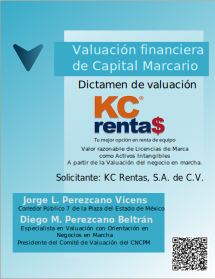
\includepdf[pages=-]{../0.portadas_eng/portada}

%-------------------------Índice-------------------------------
\newpage
\setcounter{page}{1}
\thispagestyle{fancy}
\tableofcontents

\newpage


\chapter{BACKGROUND.}\label{cap:1}
\thispagestyle{fancy}
%--------------------Datos del Valuador------------------
\section{EXPERT APPRAISER INFORMATION}\label{sec:a}

En la \lugarInforme{}, a los \numberstringnum{\diainforme} d\'ias del mes de \monthname[\mesinforme] del a\~no \numberstringnum{\annoinforme}, Yo, \textbf{\textcolor{principal}{\nombrePerito, \descripcionPerito}}; en mis funciones de PERITO VALUADOR que la Ley  me otorga; con base en mis conocimientos t\'ecnicos y mediante la aplicaci\'on de t\'ecnicas de valuaci\'on, seg\'un lo dispuesto por el art\'iculo 6, fracci\'on II y dem\'as relativos de la Ley Federal de Corredur\'ia P\'ublica; art\'iculos 6, segundo p\'arrafo, 56 Bis del Reglamento de la Ley Federal de Corredur\'ia P\'ublica; expido a continuaci\'on el presente dictamen de \tipoAvaluo.

%En la \lugarInforme{}, a los \numberstringnum{\diainforme} d\'ias del mes de \monthname[\mesinforme] del a\~no \numberstringnum{\annoinforme}, Yo, \textbf{\textcolor{principal}{\nombrePerito, \descripcionPerito}}; en mis funciones de PERITO VALUADOR que la Ley  me otorga; con base en mis conocimientos t\'ecnicos y mediante la aplicaci\'on de t\'ecnicas de valuaci\'on, seg\'un lo dispuesto por el art\'iculo 6, fracci\'on II y dem\'as relativos de la Ley Federal de Corredur\'ia P\'ublica; art\'iculos 6, segundo p\'arrafo, 56 Bis del Reglamento de la Ley Federal de Corredur\'ia P\'ublica; expido a continuaci\'on la presente Opini\'on de Razonabilidad respecto de la \tipoAvaluo.
%------------------Datos del solicitante-----------------
\section{APPLICANT INFORMATION}\label{sec:b}

The company \textcolor{principal}{\empresaSolicitante}, hereinafter referred to as \textcolor{principal}{``\empresaCorto''}, represented by \textcolor{principal}{\personaSolicitante} in his capacity as \textcolor{principal}{\caracterSolicitante}.



\espacio{3cm}

\chapter{DATA OF THE ASSET SUBJECT TO VALUATION}\label{cap:2}
\thispagestyle{fancy}
\setcounter{section}{2}
%-----------------Datos del Propietario----------------
\section{OWNER'S INFORMATION}\label{sec:c}
El titular del activo intangible sujeto de valuación es  la sociedad \textcolor{principal}{\empresaSolicitante}\\

El solicitante le declara en este acto al valuador que la sociedad 
\textcolor{principal}{\empresaSolicitante} realiza el aprovechamiento de los beneficios econ\'omicos que genera el activo intangible; cuyos flujos de efectivo se reflejan en los estados financieros.\\

\textit{\underline{Nota}: El perito valuador no llev\'o a cabo una revisi\'on independiente respecto a la titularidad del activo intangible, por lo que este dictamen no se puede considerar como un due diligence o una auditor\'ia de propiedad intelectual.}
%-----------------Tipo de servicio de valuación------
\section{TYPE OF VALUATION SERVICE}\label{sec:d}
A petici\'on del solicitante se llev\'o a cabo un avalúo de \textcolor{principal}{\tipoAvaluo}.

%-----------------Vigencia-----------------------------
\section{REPORT VALIDITY}\label{sec:e}



The validity of this report is  \textcolor{terciario}{\vigenciaInforme{}} \footnote{In the absence of specific provisions regarding the validity of this type of valuation report, the one-year term mentioned in Article 3 of the Regulation of the Federal Fiscal Code was used.}.\\[5pt]


\textcolor{secundario}{Extrinsic or administrative validity:} The validity of an appraisal is determined by its purpose or intended use and depends on the time frame established, if applicable, by the competent authority or administrative institution utilizing the report.\\[10pt]


\noindent\textcolor{secundario}{Intrinsic validity:} A report will remain valid as long as there are no substantial changes in the fundamental conditions and premises that supported the calculation (\textit{ceteris paribus}). Any substantial changes could potentially affect the reliability of the conclusive figures of the valuation.\\


%---------------Descripción de los bienes Sujetos de valuación-----------
\section{DESCRIPTION OF THE VALUATION SUBJECT}\label{sec:f}
\begin{enumerate}[\thesection.1.]
\item El solicitante le proporcion\'o al valuador el t\'itulo de registro de la marca registrada \textcolor{principal}{\marca{}} la cual es explotada y/o tiene relaci\'on con los flujos de ingresos de la sociedad \textcolor{principal}{\empresaSolicitante}; misma que se detalla y se agrega al \textcolor{terciario}{AP\'ENDICE 1:}

\begin{figure}[H]
\centering
\includegraphics[width=12cm]{../0.imagenes/bien_1}\\
\end{figure}

\end{enumerate}

\textit{\underline{Nota 1}: El presente dictamen no consiste en una auditor\'ia de propiedad intelectual respecto de los derechos mencionados anteriormente, ni se puede considerar como un due diligence de propiedad intelectual de la marca mencionada por el solicitante; por lo que se asume como informaci\'on precisa y de buena fe, seg\'un se relaciona en la semblanza de la empresa que se agrega a este informe como \textcolor{terciario}{AP\'ENDICE 2.}}\\

\textit{\underline{Nota 2}: El valuador y su perito auxiliar no asumen responsabilidad alguna respecto de errores o imprecisiones en la informaci\'on mencionada en este inciso y su relaci\'on con los ingresos de la empresa sujeta de valuaci\'on que explota los beneficios de dichos activos intangibles; seg\'un se aprecia en sus estados financieros.}

%-----------------Ubicación del bien sujeto de valuavión
\section{LOCATION OF THE VALUATION SUBJECT}\label{sec:g}
La sociedad \textcolor{principal}{\empresaCorto}, con RFC \textcolor{peincipal}{\rfcEmpresa}, tiene su domicilio fiscal ubicado en \textcolor{principal}{\ubicacionBien.}
%-----------------Propósito----------------------
\section{VALUATION PURPOSE}\label{sec:h}
Estimar el Valor Razonable (\textit{\gls{fairvalue}}) del portafolio de activos intangibles mencionado en el punto \ref{portafolio}, con fecha de valores a \fechaValores.
%------------------Uso de la valuación---------------
\section{VALUATION USE}\label{sec:i}


The applicant has informed the Appraiser that they require this report for \textcolor{principal}{\usoAvaluo}.



\newpage

\chapter{LEGAL BASIS AND PRELIMINARY CONSIDERATIONS.}\label{cap:3}
\thispagestyle{fancy}
\setcounter{section}{9}

\section*{LEGAL BASIS.}\label{sec:juridico}
The present analysis, as well as the opinions and conclusions of the undersigned appraiser, were developed in accordance with Article 6, Section II of the Federal Public Brokerage Law (LFCP), Article 56 bis of its regulations, international valuation standards, and the theoretical framework of corporate finance.\\

The following are various legal bases in Mexican regulations related to valuation reports:\\


\textcolor{principal}{Código de Comercio:}\\[10pt]

\textit{``Artículo 1252.- Los peritos deben tener título en la ciencia, arte, técnica, oficio o industria a que pertenezca la cuestión sobre la que ha de oírse su parecer, si la ciencia, arte, técnica, oficio o industria requieren título para su ejercicio.}\\[10pt]

\textit{Si no lo requirieran o requiriéndolo, no hubiere peritos en el lugar, podrán ser nombradas cualesquiera personas entendidas a satisfacción del juez, aun cuando no tengan título.}\\

\textit{La prueba pericial sólo será admisible cuando se requieran conocimientos especiales de la ciencia, arte, técnica, oficio o industria de que se trate, más no en lo relativo a conocimientos generales que la ley presupone como necesarios en los jueces, por lo que se desecharán de oficio aquellas periciales que se ofrezcan por las partes para ese tipo de conocimientos, o que se encuentren acreditadas en autos con otras pruebas, o tan sólo se refieran a simples operaciones aritméticas o similares.} \\[10pt] 

\textit{El título de habilitación de corredor público acredita para todos los efectos la calidad de perito valuador.''} (...)\\[10pt]

\textit{``Artículo 1257.- Los jueces podrán designar peritos de entre aquéllos autorizados como auxiliares de la administración de justicia por la autoridad local respectiva, o a solicitar que el perito sea propuesto por colegios, asociaciones o barras de profesionales, artísticas, técnicas o científicas o de las instituciones de educación superior públicas o privadas, o las cámaras de industria, comercio, o confederaciones de cámaras a la que corresponda al objeto del peritaje.  (...)''}\\[10pt]

\textit{``Artículo 1300.- Los avalúos harán prueba plena.}\\[10pt]


\textcolor{principal}{LEY FEDERAL DE CORREDUR\'IA P\'UBLICA}\\[10pt]

\textit{``ARTICULO 6o.- Al corredor público corresponde: (...)}\\[10pt]

\textit{II.- Fungir como perito valuador, para estimar, cuantificar y valorar los bienes, servicios, derechos y obligaciones que se sometan a su consideraci\'on, por nombramiento privado o por mandato de autoridad competente; (...)}\\[10pt]

\textit{VIII. Las dem\'as funciones que le señalen \'esta y otras leyes o reglamentos.}\\[10pt]

\textit{Las anteriores funciones se entender\'an sin perjuicio de lo dispuesto en otras leyes y no se consideran exclusivas de los corredores p\'ublicos.'' }\\[10pt]




\textcolor{principal}{REGLAMENTO DE LA LEY FEDERAL DE CORREDUR\'IA P\'UBLICA}\\


``\textcolor{secundario}{ARTICULO 56 Bis.-} \textit{El corredor p\'ublico en ejercicio de sus funciones como perito valuador, podr\'a estimar, cuantificar y valorar los bienes, servicios, derechos y obligaciones que se sometan a su consideraci\'on por nombramiento privado o por mandato de autoridad competente.} \\

\textit{El informe de valuaci\'on debe formularse de manera clara y objetiva, presentando el razonamiento y la informaci\'on suficiente con las cuales se obtiene el valor conclusivo del bien, servicio, derecho u obligaci\'on, y deber\'a contener cuando menos los siguientes rubros enunciativos: }

\begin{enumerate}[a)]

\item Nombre completo, n\'umero y plaza del Corredor as\'i como su firma y sello; 
\item Datos del solicitante; 
\item Datos del propietario, indicando en su caso la informaci\'on en que se basa; 
\item Tipo de servicio de valuaci\'on; 
\item Vigencia del aval\'uo, siendo este requisito obligatorio cuando exista una disposici\'on legal que as\'i lo establezca; 
\item Descripci\'on del bien, derecho, servicio u obligaci\'on materia del aval\'uo; 
\item  Cuando proceda, ubicaci\'on del bien materia de la valuaci\'on; 
\item Prop\'osito del informe de valuaci\'on; 
\item Uso del informe de valuaci\'on; 
\item Consideraciones previas a la valuaci\'on; 
\item Descripci\'on de enfoques de valuaci\'on aplicados; 
\item Fecha de la Inspecci\'on; 
\item En su caso fecha de referencia de valor; 
\item Fecha del informe de valuaci\'on; 
\item Fuentes de informaci\'on; 
\item Consideraciones previas a la conclusi\'on; 
\item Conclusi\'on de valor; 
\item Reporte fotogr\'afico, y 
\item En su caso, anexos. 

\end{enumerate}

\textit{Cualquier observaci\'on respecto a enfoques, fuentes de informaci\'on, elementos, limitaciones generales, entre otros, que incidan en la conclusi\'on del valor, deber\'an ser mencionadas en el informe.} \\

\textit{Cuando en raz\'on del servicio valuatorio, territorio, prop\'osito, uso u objeto del dictamen solicitado al corredor se desprenda que, con base en una normatividad particular expedida por autoridad competente que sea de car\'acter obligatorio, deba expedir o elaborar el dictamen utilizando leyes, normas, lineamientos, manuales o reglas espec\'ificas, el corredor podr\'a optar por sujetarse \'unicamente a dicha normatividad.} \\

\textit{Trat\'andose de remates, aval\'uos para efectos judiciales o procedimientos administrativos o aval\'uos solicitados por autoridades donde sea f\'isica o materialmente imposible realizar la inspecci\'on f\'isica del bien objeto de valuaci\'on, u obtener del solicitante o propietario la documentaci\'on correspondiente, se deber\'a se\~nalar expresamente en el dictamen y se realizar\'a el aval\'uo con los datos e informaci\'on de los que pueda allegarse el Corredor en el momento con los medios a su alcance.}''\\



\textcolor{principal}{AGREEMENT ESTABLISHING GUIDELINES FOR PUBLIC BROKERS TO ISSUE APPRAISALS ISSUED BY THE SECRETARY OF COMMERCE AND INDUSTRIAL PROMOTION, PUBLISHED IN THE OFFICIAL GAZETTE ON MARCH 9, 1999.}\\[10pt]



\textit{``Article 2.- The valuation report issued by the public broker shall be composed of the following sections:}

\begin{enumerate}[I.]

\item Background;
\item Data of the asset or service subject to valuation; 
\item Legal basis and preliminary considerations; 
\item  Methodology employed;
\item  Development of the appraisal, and
\item  Conclusions.

\end{enumerate}

\textit{Furthermore, in all cases, the public broker must have complete documentary support regarding the market study conducted for the purposes of the appraisal. (...)}\\[10pt]

\textit{Article 12.- In valuations performed by public brokers for intangible assets, considering their nature or type, their values may be determined as follows:}

\begin{enumerate}[I.-]
\item By researching the market for similar or substitute goods and products based on commercial references, implied and calculated values, considering sales volumes and profitability, possible purchase and sale cases, or alternatively, royalty payments for the use and exploitation of patents, trademarks, or franchises;

\item In the case of projects, an analysis will be conducted of the infrastructure of services available, marketing characteristics, technology used, price determination, investment costs, loss of profit, financial performance, and profit margins, in order to diagnose their investment margins, cash flows, and break-even points;

\item Through the study of the best utilization of projects and the commercial value of real or potential gross rents generated, as well as calculating the equivalent capital capable of providing those rents under non-inflationary and low-risk conditions, considering whether it is a project valuation or an ongoing business, or

\item When it comes to transfer pricing, it shall be done by applying the procedures established in the Income Tax Law or, alternatively, using the appropriate method for the case. (...)''

\end{enumerate}
%---------------Consideraciones previas a la valuaci\'on--------------------
\section{PRIOR CONSIDERATIONS FOR VALUATION}\label{sec:j}

	\subsection{Conditions, Restrictions, and Limitations of the Report:}
\subsection{Condiciones, restricciones y limitantes del informe}

\begin{enumerate}[\indent a)]
\item Se asume que este avalúo atiende a una solicitud de prestación de servicios profesionales cuyo sustento es la buena fe entre las partes; en este caso, el solicitante y el Perito Valuador; por tal motivo, la información verbal y escrita que en su caso, ha sido proporcionada, se entiende que es correcta a saber a la fecha del presente avalúo, además de manifestar el solicitante que no cuenta con información adicional  que pudiese afectar los valores que se expresan en el presente dictamen.

\item Después de haber llevado a cabo la lectura total del presente avalúo, el solicitante declara que no contempla situaciones subyacentes, ocultas o extraordinarias que en su momento no hubiesen sido debidamente reportadas al suscrito.

\item La propiedad legal no fue verificada, ni la existencia de gravámenes y/o reservas de dominio sobre el bien valuado. No se considera para la determinación del presente valor razonable, gravamen alguno sobre el activo intangible objeto de la valuación.

\item El presente documento se limita a una estimación de valor de activos intangibles, con base en los modelos de valuación expuestos en su capítulo respectivo, salvo error u omisión. Lo anterior se fundamenta en las propias variaciones de los modelos y el entorno económico y en consecuencia como limitante, las suposiciones de razones fundamentales para su proyección y cálculos realizados con base en la información recibida.

\item No se verificó, ni se consideró para la determinación del valor conclusivo, una revisión legal o \textit{due diligence} de la titularidad del activo intangible, cuyos beneficios económicos controla actualmente sociedad \textcolor{principal}{\empresaSolicitante.} El presente dictamen no puede ser considerado como un reporte de auditoría en ese sentido. 

\item El presente dictamen se expide exclusivamente para la fecha contenida en este reporte, con fecha de valores  al \textcolor{principal}{\fechaValores}. Podrían existir cambios a partir de dicha fecha en factores externos o internos de la sociedad sujeta de análisis en sus cifras financieras; que pudieren afectar el valor conclusivo contenido en el presente dictamen.

\item Para la práctica de este avalúo únicamente se valoraron y estudiaron las cifras proporcionadas por el solicitante, así como los documentos a que se ha hecho mención en el \autoref{sec:nn} de este dictamen. Asimismo, el solicitante manifestó, a través de su representante legal, que no cuenta con información adicional que pudiera servir de base para modificar las cifras aquí señaladas. En el mismo sentido, no se ha efectuado una revisión independiente respecto del contenido y veracidad de dicha documentación y el análisis y resultados podrían verse afectados en caso de que dicha información no sea correcta y/o precisa.

\item La información recibida por el perito valuador para su análisis, corresponde a información relevante de la empresa cuyo activo intangible fue sujeto de valuación, por lo que se asume el carácter de confidencialidad de la misma y se limita su uso para el presente informe.

\item Todos los criterios utilizados para la valuación descartan cualquier cuestionamiento especulativo o particular en un momento dado. Se asume la pertenencia del activo intangible y de la empresa de acuerdo a la situación actualmente conocida. Asimismo, se asumen como constantes los comportamientos actuales del mercado (\textit{ceteris paribus}).

\item Las proyecciones realizadas para la estimación de valor a que se refiere el presente documento no son predicciones del futuro; son el mejor estimado del perito valuador sobre las condiciones actuales proyectadas en el futuro respecto de las cifras financieras de la sociedad. El perito valuador no puede garantizar que dichos pronósticos y estimaciones se materializarán.

\item Los análisis, opiniones y conclusiones reportadas están limitadas por las suposiciones y condiciones limitantes señaladas, y son mis propios análisis, opiniones y conclusiones profesionales e imparciales.

\item Se toman como ciertas las declaraciones realizadas por el solicitante del presente dictamen valuatorio. El suscrito no asume responsabilidad alguna sobre la veracidad y exactitud del dicho e información proporcionada por el solicitante.

\item No debe considerarse que el valor conclusivo del presente dictamen valuatorio sea necesariamente el precio o la contraprestación que deba fijarse para la venta, compra, enajenación, registro, cesión o transmisión del bien objeto de la valuación  contenida en este documento.

\item El presente dictamen valuatorio no debe ser considerado necesariamente como una recomendación para la venta, compra, enajenación, cesión, transmisión o constitución de garantía de los bienes objeto del mismo; ni para llevar a cabo algún tipo de negocio, inversión u operación con el mismo.

\item El presente dictamen valuatorio fue preparado para \textcolor{principal}{\empresaSolicitante}{} y su destino está limitado para el uso especificado  en el mismo. Conforme a lo anterior, el perito valuador no asume responsabilidad alguna frente a terceros por el contenido del presente dictamen valuatorio. El perito valuador no da ni ofrece garantía alguna a terceros (incluyendo inversionistas) respecto del contenido del presente dictamen valuatorio.

\item Este dictamen valuatorio sólo podrá ser usado integro y no en partes. Ninguna parte del reporte podrá ser utilizada en conjunto a algún estudio ajeno al mismo. La publicación de este dictamen valuatorio o cualquiera de sus partes, sin la autorización escrita del perito valuador está prohibida. Asimismo, este dictamen valuatorio no podrá ser usado por ninguna entidad distinta a la que esté dirigida o para un propósito o uso distinto al estipulado.

\end{enumerate}
\textcolor{principal}{DEFINICIONES Y CONCEPTOS.}

\begin{enumerate}[\indent\itshape a)]
\item \textcolor{principal}{\textit{CAPITAL CONTABLE }}

\textit{Es la diferencia entre los activos y pasivos de la empresa y está constituido por la suma de todas las cuentas de capital, es decir, incluye capital social, reservas, utilidades acumuladas y utilidades del ejercicio.}

\item \textcolor{principal}{\textit{CAPITAL INVERTIDO}}

\textit{Son los bienes que constituyen el Activo Tangible de una Sociedad. El Capital Invertido por lo general refleja el desembolso realizado por los inversionistas para iniciar una Empresa y las adiciones de Capital realizadas durante su funcionamiento. Regularmente su cálculo corresponde al Activo Total menos Pasivo Circulante o en segunda forma al Activo No Circulante más Capital de Trabajo.}

\item  \textcolor{principal}{\textit{FECHA DE REPORTE}}

\textit{Corresponde a la fecha en que fue realizado y firmado el documento de valuación. Puede ser igual o distinta a la fecha de valores.}

\item  \textcolor{principal}{\textit{FECHA DE VALORES}}

\textit{Es la fecha que el valuador asentar\'a al momento del cierre de valores en su trabajo valuatorio. Puede ser igual o distinta a la fecha del reporte.}

\item \textcolor{principal}{ \textit{PROP\'OSITO DEL AVAL\'UO}}

\textit{Es la intenci\'on expresa de determinar un tipo de valor que ser\'a estimado en funci\'on de los bienes a valuar, a la especialidad valuatoria y al uso del aval\'uo se\~nalado por el solicitante.}

\item \textcolor{principal}{\textit{USO DEL AVAL\'UO}}

\textit{Es el destino que se le pretende dar al dictamen y que expresamente se\~nala el solicitante del servicio.}


\item  \textcolor{principal}{\textit{VALOR EN LIBROS}}

\textit{Es el importe con que un rengl\'on contable aparece registrado en los libros de contabilidad, ya sea que represente el costo, inicial, el actualizado, el estimado o el de aval\'uo. Representa el valor con que se registra en los libros de contabilidad cualquier propiedad, derecho, bien, cr\'edito u obligaci\'on. El valor en libros representa \'unicamente ``cifras en libros'' y eso puede ser diferente del valor comercial, del valor en el mercado, del valor real, del valor de reposici\'on, del valor de liquidaci\'on, etc.}

\item \textcolor{principal}{\textit{VALOR DE REALIZACI\'ON ORDENADA}}

\textit{Es el precio estimado que podr\'ia ser obtenido a partir de una venta en el mercado libre, en un periodo de tiempo apenas suficiente para encontrar un comprador o compradores, en donde el vendedor tiene urgencia de vender, donde ambas partes act\'uan con conocimiento y bajo la premisa de que los bienes se venden en el lugar y en el estado en que se encuentran.}

\item \textcolor{principal}{ \textit{VALOR DE LIQUIDACI\'ON FORZADA}}

\textit{Es la cantidad bruta, expresada en t\'erminos monetarios, que se espera obtener por concepto de una venta p\'ublica debidamente anunciada y llevada a cabo en el mercado abierto, en la que el vendedor se ve en la obligaci\'on de vender de inmediato por mandato judicial ``tal como est\'a y donde se ubica'' el activo. En algunos casos, puede involucrar un vendedor no deseoso y un comprador o compradores que compran con conocimiento de la desventaja para el vendedor.}

\item \textcolor{principal}{ \textit{VALOR RAZONABLE}}

\textit{Conforme a su definici\'on insertada en la publicaci\'on de NIIF, (IAS) International Accounting Standards Committee Foundation y por el (IMCP) Instituto Mexicano de Contadores P\'ublicos, que a la letra indica (sic)  `...El importe por el que puede ser intercambiado un activo o cancelado un pasivo, entre partes interesadas y debidamente informadas, en una transacción realizada en condiciones de independencia mutua…''}

\end{enumerate}


\subsection{VALUATION APPROACHES}

In practice, there are three generally accepted valuation approaches to estimate the fair value of an ongoing business, investment project, and its tangible and intangible assets. These approaches are briefly described below:

\begin{figure}[H]
\centering
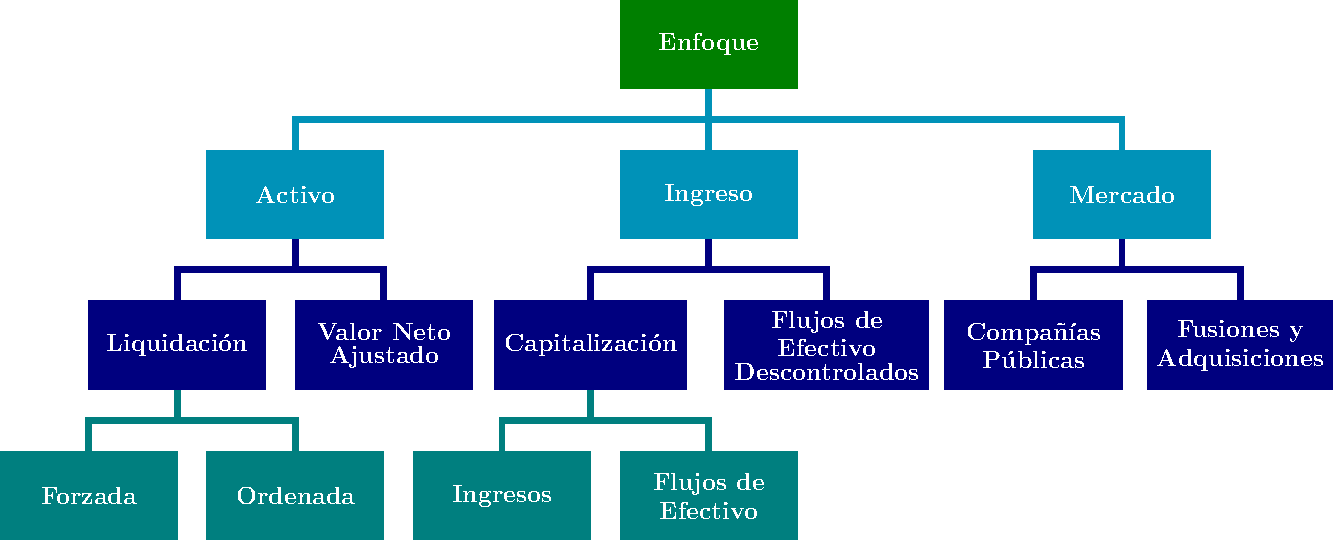
\includegraphics[width=14cm]{\rutaImagenes/enfoques_mas_utilizados_eng}
\end{figure}

\subsubsection{Asset Approach}

The asset approach is a general way to determine the fair value of a company's equity, a business, investment project, tangible asset, or intangible asset using one or more methods based on the value of assets and their net liabilities.\\[10pt]

In business valuation, the asset approach can be considered equivalent to the cost approach in other valuation disciplines. \\[10pt]

There are two general methods in the asset approach for business valuation:\\[10pt]

\textcolor{secundario}{Adjusted Book Value Method:} This method adjusts assets and liabilities (including off-balance sheet items, intangibles, and contingent liabilities) to their market value.\\[10pt]

\textcolor{secundario}{Excess Earnings Capitalization Method:} This method involves a revaluation of all the assets and liabilities of the company. This method is not used to determine the total value of a business but to determine the value of goodwill or intangible assets.\\[10pt]

It is important to distinguish between the application of a valuation method within the asset approach and the ``book value''. Under any valuation standard, the fact that the market value of a business or company is equal to its book value would be a coincidence or would depend on very particular circumstances of the entity being valued.\\[10pt]

\subsubsection{Market Approach}

The market approach determines the fair value of a company's equity, business, investment project, tangible asset, or intangible asset by using methods that compare the appraised asset with similar assets.\\[10pt]

The business, shares, tangible assets, or intangible assets used for comparison should be reasonably similar to the appraised asset. Key factors to consider in determining comparability include:\\[10pt]

\begin{itemize}

\item Sufficient similarity in quantitative and qualitative characteristics.

\item The amount and verifiability of information regarding the asset.

\item Whether the price of the similar asset was determined in a transaction between independent parties, i.e., in a voluntary sale between the parties.

\item Comparisons are generally made using valuation ratios (multiples); the calculation and use of these ratios should provide a significant reference regarding the value of the asset, considering all relevant factors.

\end{itemize}

Methods in the market approach include:\\[10pt]

\textcolor{secundario}{Public Company Guideline Method:} This method determines market multiples of stock prices of publicly traded companies (listed on a stock exchange) with a similar line of business to the appraised company.\\[10pt]

\textcolor{secundario}{Transaction Guideline Method:} This method determines market multiples of similar transactions completed between independent parties.\\[10pt]

\subsubsection{Income Approach}

The income approach is a general way to determine the fair value of a company's equity, business, asset, or intangible asset using one or more methods by which economic benefits are converted into value.\\[10pt]

In the income approach, anticipated benefits are expressed in monetary terms and can be reasonably represented by concepts such as dividends or distributions, various types of earnings, or cash flows.\\[10pt]

To estimate anticipated benefits, elements such as capital structure, historical performance of the entity, the future industry environment, and economic factors must be considered.\\[10pt]

Anticipated benefits are converted into value through procedures that consider expected growth and timing of benefits, as well as the risk profile of the benefits and the time value of money.\\[10pt]

Typically, converting anticipated benefits into value requires determining a capitalization rate or discount rate. To determine these rates, factors such as interest rate levels, expected rates of return by investors in alternative investments, and specific risk characteristics of anticipated benefits must be considered.\\[10pt]






\newpage
\begin{center}
	\underline{\textbf{\textcolor{principal}{ACR\'ONIMOS}}}
\end{center}

\begin{table}[H]
 	\begin{tabular}{rp{10cm}}
\textit{Beta}:&	El coeficiente Beta ($\beta$) es una medida de volatilidad que estima el riesgo sistem\'atico de un activo.\\
\textit{CAGR}:&	Tasa compuesta de crecimiento anual.\\
\textit{CAPM}:&	Modelo de valoraci\'on de Activos de Capital.\\
\textit{Cash \& Eq.}:&	Efectivo y Equivalentes.\\
\textit{DCF}:&	Flujo de efectivo descontado, siglas de \textit{Discounted Cash Flow}.\\\textit{Effective Tax Rate:}&	Tasa fiscal efectiva.\\
\textit{Enterprise value}:&	Valor de la empresa.\\
\textit{Equity value}:&	Valor del capital accionario.\\
\textit{Exp. Debt}:& 	Deuda expl\'icita.\\
\textit{ERP}:	& Premio de mercado.\\
\textit{Fair Value}:&	Valor razonable o valor justo de mercado.\\
\textit{FCFF}:&	Flujo de efectivo libre a la Firma, siglas de \textit{Free Cash Flow to Firm}.\\
\textit{Firm value}:&	Valor de la firma o empresa.\\
\textit{Growth Rate (G):}&	Tasa de Crecimiento de ingresos netos.\\
\textit{Income Statement}:&	Estado de Resultados.\\
\textit{Investment Capital}:& 	Capital Invertido (IC).\\
\textit{Ke}:& 	Costo del Capital Accionario.\\
\textit{Kd}:& 	Costo de la deuda.\\
%\textit{KPI}:&	Indicador clave de desempe\~no o indicadores de gesti\'on (\textit{Key Performance Indicator}).\\
\textit{Levered beta}:& 	Beta apalancada.\\
\textit{Market approach}:& 	Enfoque de mercado.\\
\textit{MPEEM}:&	Multi-Period Excess Earnings Method.\\
\textit{NCA}:&	Activo No Corriente.\\
\textit{Net Debt}:& 	Deuda neta.\\
\textit{Nopat}:& 	Flujo de Operaci\'on Neto.\\
\textit{NWC}:&	Capital de Trabajo Neto.\\
\textit{PEERS}:&	M\'ultiplos de Cotizaci\'on.\\
\textit{RFR}:& M\'etodo de Flujo de Ahorro en Regal\'ias\\
\textit{Risk free rate}:&	  Tasa Libre de Riesgo.\\
%\textit{Size prime}:&	Prima por tama\~no.\\
\textit{Terminal value}:&	Valor terminal.\\
\textit{Total Debt}:&	Deuda total.\\
\textit{Value drivers}:&  	Elevadores de Valor.\\
\textit{WACC}:& 		Costo Promedio Ponderado de Capital.\\
\textit{WARA}:&	 Costo Promedio Ponderado de Activos.\\


	\end{tabular}
\end{table}
\newacronym{cagr}{CAGR}{Tasa compuesta de crecimiento anual}
\newacronym{capm}{CAPM}{Modelo de Valoraci\'on de Activos de Capital}
\newacronym{chic}{CHIC}{Sociedades de Inversi\'on Cerradas}
\newacronym{crp}{CRP}{Riesgo Pa\'is}

\newacronym{dcf}{DCF}{Flujo de efectivo descontado (Discounted Cash FLow)}
\newacronym{erp}{ERP}{Premio de Mercado}
\newacronym{etr}{ETR}{Tasa Fiscal Efectiva}
\newacronym{fcff}{FCFF}{Flujo de efectivo libre a la Firma (Free Cash Flow to Firm)}
\newacronym{fcfe}{FCFE}{Flujo de efectivo libre al Capital (Free Cash Flow to Equity)}
\newacronym{g}{G}{Tasa de Crecimiento de ingresos netos (Grow Rate)}
\newacronym{ke}{Ke}{Costo de Capital Accionario}
\newacronym{kd}{Kd}{Costo de la deuda}
\newacronym{kpi}{KPI}{Indicador clave de desempe\~no o indicadores de gesti\'on \textit{(Key Performance Indicator)}}
\newacronym{mpeem}{MPEEM}{Multi-Period Excess Earnings Method}
\newacronym{nav}{NAV}{Valor neto de activos}
\newacronym{nca}{NCA}{Activo No Corriente}
\newacronym{nwc}{NWC}{Capital de Trabajo Neto}
\newacronym{peers}{PEERS}{M\'ultiplos de Cotizaci\'on}
\newacronym{rfr}{RFR}{M\'etodo de Flujo de Ahorro en Regalias}
\newacronym{wacc}{WACC}{Costo Promedio Ponderado de Capital}
\newacronym{wara}{WARA}{Costo Promedio Ponderado de Activos}
\newglossaryentry{beta}
{
        name=Beta ($\beta$),
        plural=Betas,
        description={El coeficiente Beta ($\beta$) es una medida de volatilidad que estima el riesgo sistem\'atico de un activo}
}

\newglossaryentry{cashNeq}
{
        name=Cash \& Eq,
        description={Efectivo y equivalentes}
}

\newglossaryentry{efectivetaxrate}
{
        name=Effective Tax Rate,
        description={Tasa fiscal efectiva}
}

\newglossaryentry{enterprisevalue}
{
        name=Enterprise value,
        description={Valor de la empresa}
}

\newglossaryentry{equityvalue}
{
        name=Equity value,
        description={Valor del capital accionario}
}

\newglossaryentry{exitmultiple}
{
        name=Exit multiple,
        description={M\'ultiplo de salida}
}

\newglossaryentry{expdebt}
{
        name=Explicit Debt,
        description={Deuda expl\'icita}
}

\newglossaryentry{fairvalue}
{
        name=Fair Value,
        description={Valor razonable o valor justo de mercado}
}

\newglossaryentry{firmvalue}
{
        name=Firm Value,
        description={Valor de la firma o empresa}
}

\newglossaryentry{growthrate}
{
        name=Growth Rate,
        description={Tasa de crecimiento de ingresos netos}
}

\newglossaryentry{incomestatement}
{
        name=Income Statement,
        description={Estado de Resultados}
}

\newglossaryentry{investmentcapital}
{
        name=Investment Capital,
        description={Capital Invertido (IC)}
}

\newglossaryentry{leveredbeta}
{
        name=beta apalancada,
        plural=betas apalancadas,
        description={Levered beta}
}

\newglossaryentry{marketaproach}
{
        name=Market approach,
        description={Enfoque de mercado}
}

\newglossaryentry{netdebt}
{
        name=Net Debt,
        description={Deuda neta}
}

\newglossaryentry{nopat}
{
        name=NOPAT,
        description={Flujo de Operaci\'on Neto}
}

\newglossaryentry{projectvaluation}
{
        name=Project Valuation,
        description={Valor razonable del proyecto de inversi\'on}
}

\newglossaryentry{riskfreerate}
{
        name=Risk Free Rate,
        description={Tasa Libre de Riesgo}
}

\newglossaryentry{sizeprime}
{
        name=Size Prime,
        description={Prima por tama\~no}
}

\newglossaryentry{terminalvalue}
{
        name=Terminal Value,
        description={Valor terminal}
}

\newglossaryentry{totaldebt}
{
        name=Total Debt,
        description={Deuda total}
}

\newglossaryentry{valuedrivers}
{
        name=Value drivers,
        description={Elevadores de Valor}
}
	
\chapter{METHODOLOGY EMPLOYED}\label{cap:4}
\thispagestyle{fancy}

The valuation of the asset mentioned in \autoref{cap:2}  \autoref{sec:f} of this report was carried out, which is explained below:

%-----------------------Descripci\'on de los enfoques de valuaci\'on aplicados-------------
\setcounter{section}{10}
\section{DESCRPTION OF APPLIED VALUATION APPROACHES.}\label{sec:k}

\renewcommand\thefigure{\arabic{figure}} 


\subsection{ESTIMATION OF FAIR VALUE:}

This report concerns the fair value of the Equity Capital (\textit{\gls{equityvalue}}) of \textcolor{principal}{\empresaSolicitante} as well as the estimation of the fair value per share; as mentioned in \autoref{sec:f}, with the valuation date of \textcolor{principal}{\fechaValores}.\\[10pt]

The appraiser received financial information from the applicant, which was analyzed in detail to understand the business plan that supports the financial analysis of the business carried out for the current equity valuation. (\textcolor{secundario}{APPENDIX 2}).\\



\subsection{POTENTIAL VALUE WITH INTERNAL OPPORTUNITIES.} 


The equity valuation of \textcolor{principal}{\empresaSolicitante} was conducted based on the business and financial information provided by the applicant, applying the theoretical framework of business valuation; under point 3 of the McKinsey Pentagon (\textit{``Value with internal improvements''}): (\textcolor{terciario}{\autoref{fig:hexagono}}).

\begin{figure}[H]
\centering
\caption{Opportunity Exploitation Pentagon \label{fig:hexagono}}\vspace{10pt}
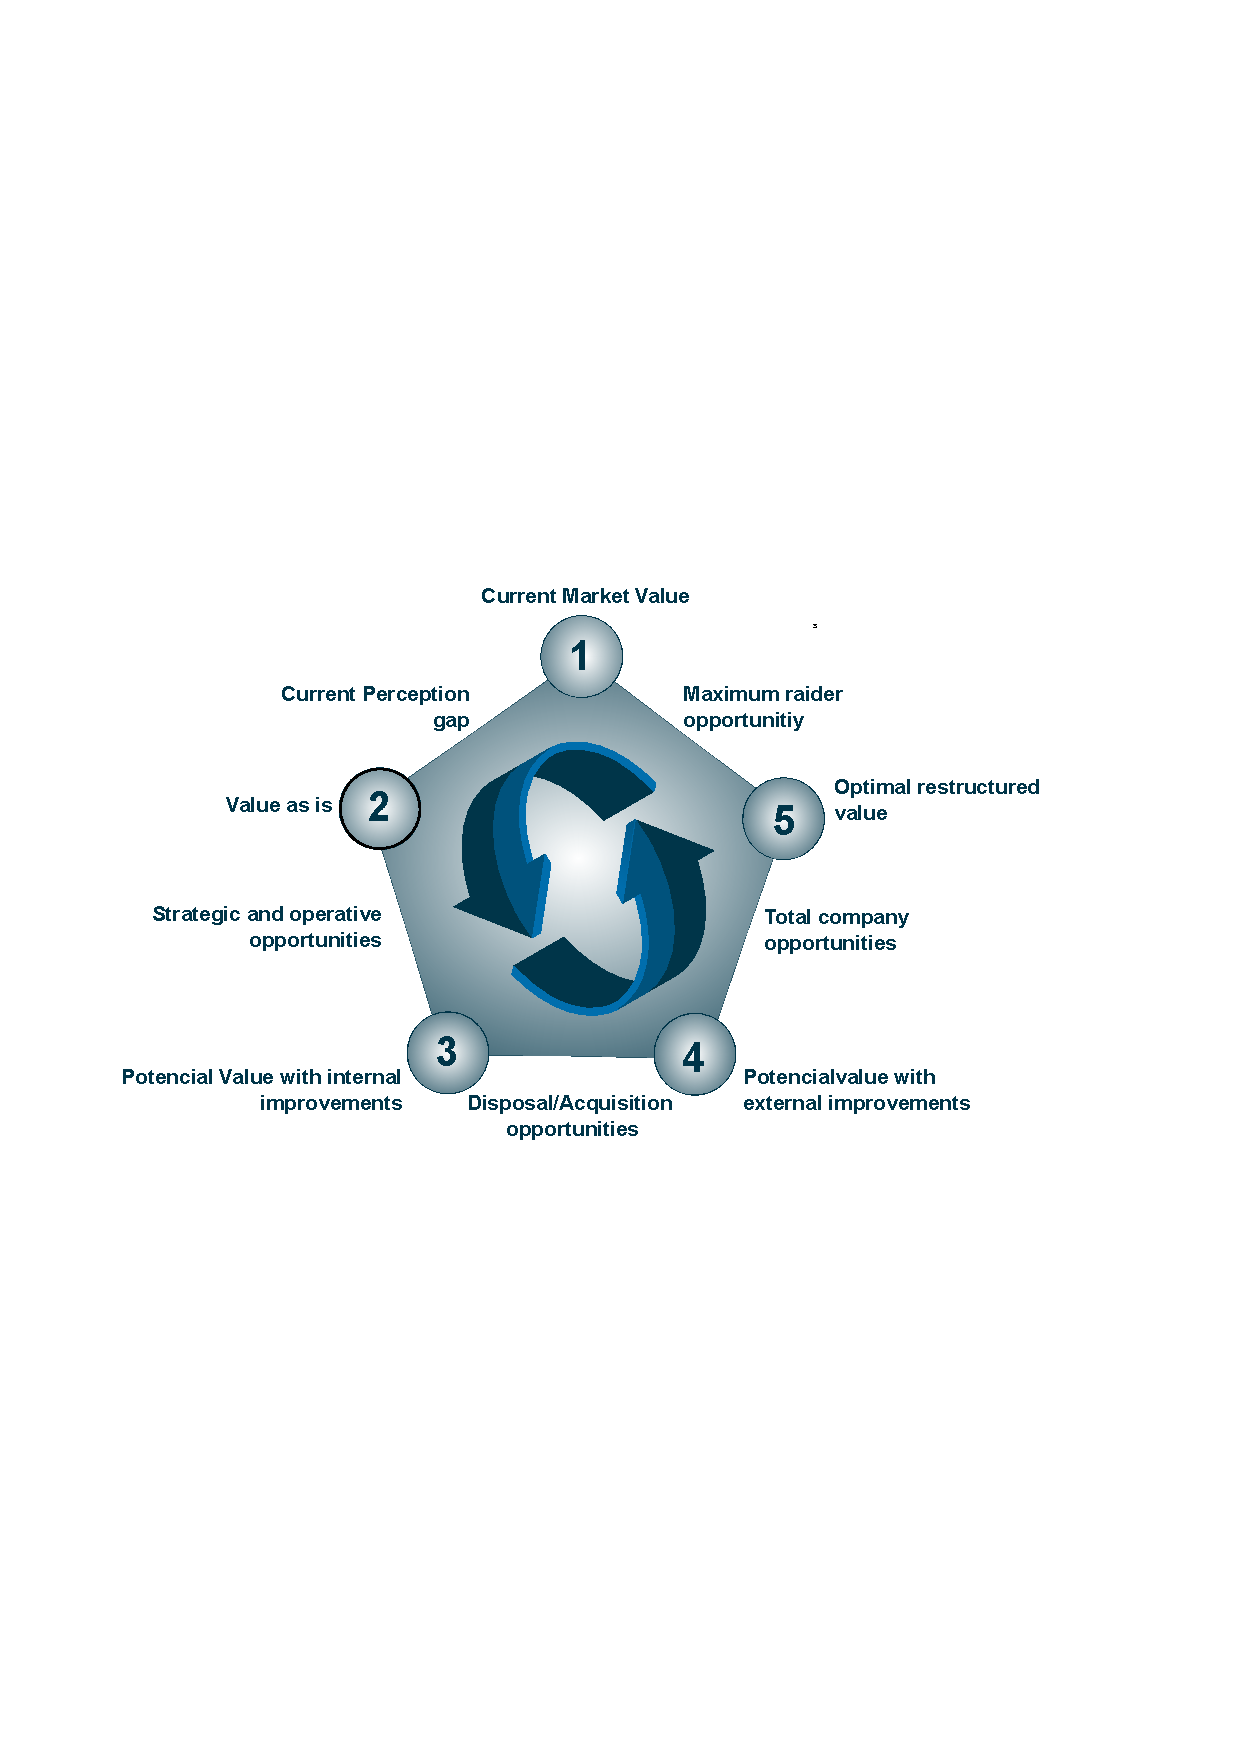
\includegraphics[width=8cm]{\rutaImagenes/penthagon}\\
Source: Valuation. Copeland Tom, Koller Tim y Murrin Jack.\\

John Wiley \& Sons. 2000.
\end{figure}

``\textcolor{secundario}{Value with internal improvements}.- It is the value acquired by the valued economic unit once the identification and exploitation of internal factors have been carried out. To achieve this, deficiencies are corrected, processes are improved and optimized, and new strategic opportunities are exploited, thus obtaining a higher value of the economic unit.''\\




\textcolor{secundario}{METODOLOG\'IAS DE VALUACI\'ON DE NEGOCIOS}. Se aplicaron dos t\'ecnicas de valuaci\'on de negocios, con amplia aceptaci\'on en el medio financiero (\autoref{fig:metodologias}), con el objeto de determinar el valor del negocio como capital invertido en uso.\\

\begin{figure}[H]
\centering
\caption{Metodolog\'ias de Valuaci\'on de Negocios m\'as utilizadas\label{fig:metodologias}}
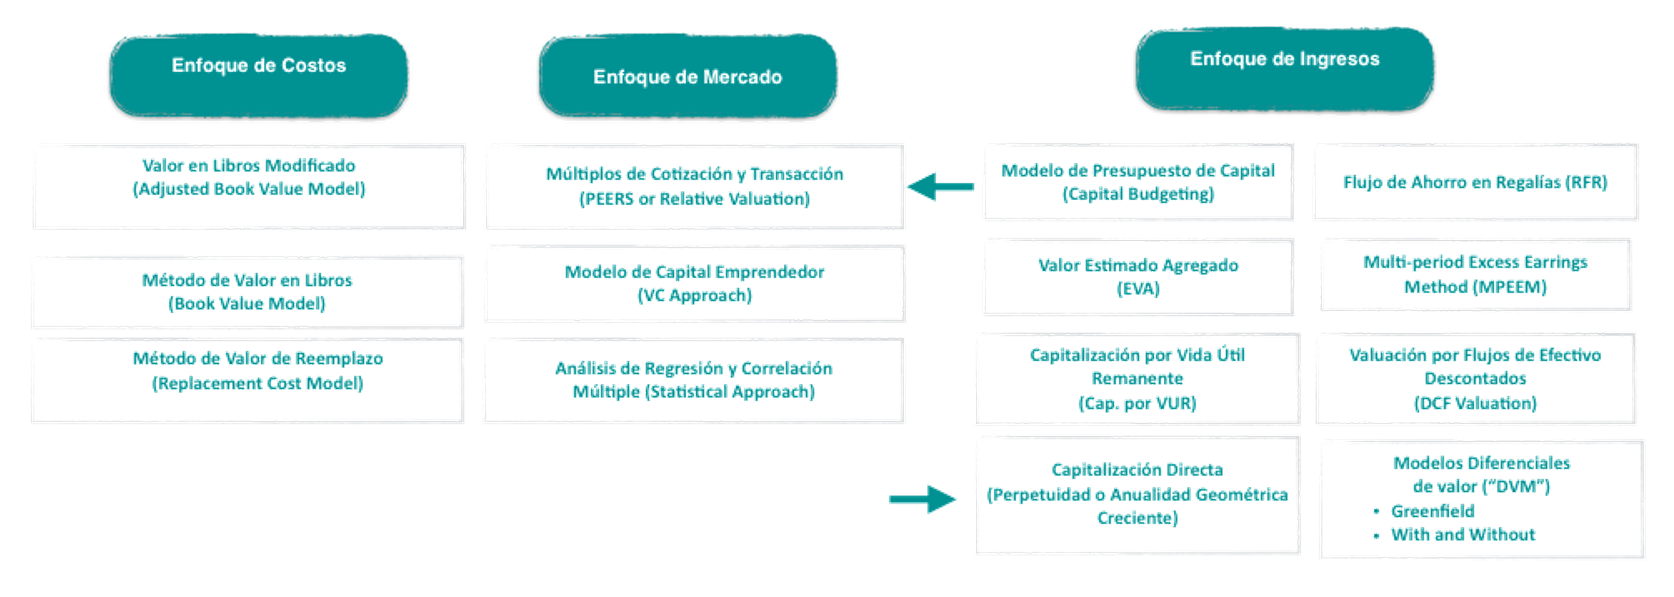
\includegraphics[width=17cm]{\rutaImagenes/metodologias_valuacion_negocio_1}\\

\end{figure}

\textcolor{secundario}{ESTIMACI\'ON DE LA TASA DE DESCUENTO}. La tasa de descuento generalmente aplicable a la estimaci\'on de activos intangibles puede ser calculada bajo los modelos financieros conocidos como  \gls{wacc} o \gls{wara}. Dicha tasa de descuento consiste en el rendimiento m\'inimo esperado para la organizaci\'on (\autoref{fig:op_acc} y \ref{fig:narr_val} ).

\begin{figure}[H]
\centering
\begin{minipage}{8cm}
\caption{Costo de oportunidad de los Accionistas\label{fig:op_acc}}
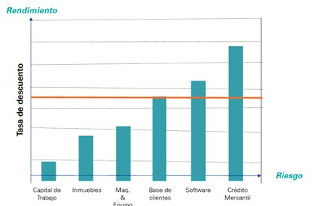
\includegraphics[height=5cm]{\rutaImagenes/costo_oportunidad_accionistas}
\footnotesize{Fuente: Valuaci\'on de Activos Intangibles. DEAL ADVISORY MEXICO. KPMG C\'ARDENAS DOSAL, S.C. KPMG ``D.R.'' \copyright 2016}
\end{minipage}
\quad
\begin{minipage}{8cm}
\caption{Fundamentos de la Narrativa Valuatoria\label{fig:narr_val}}
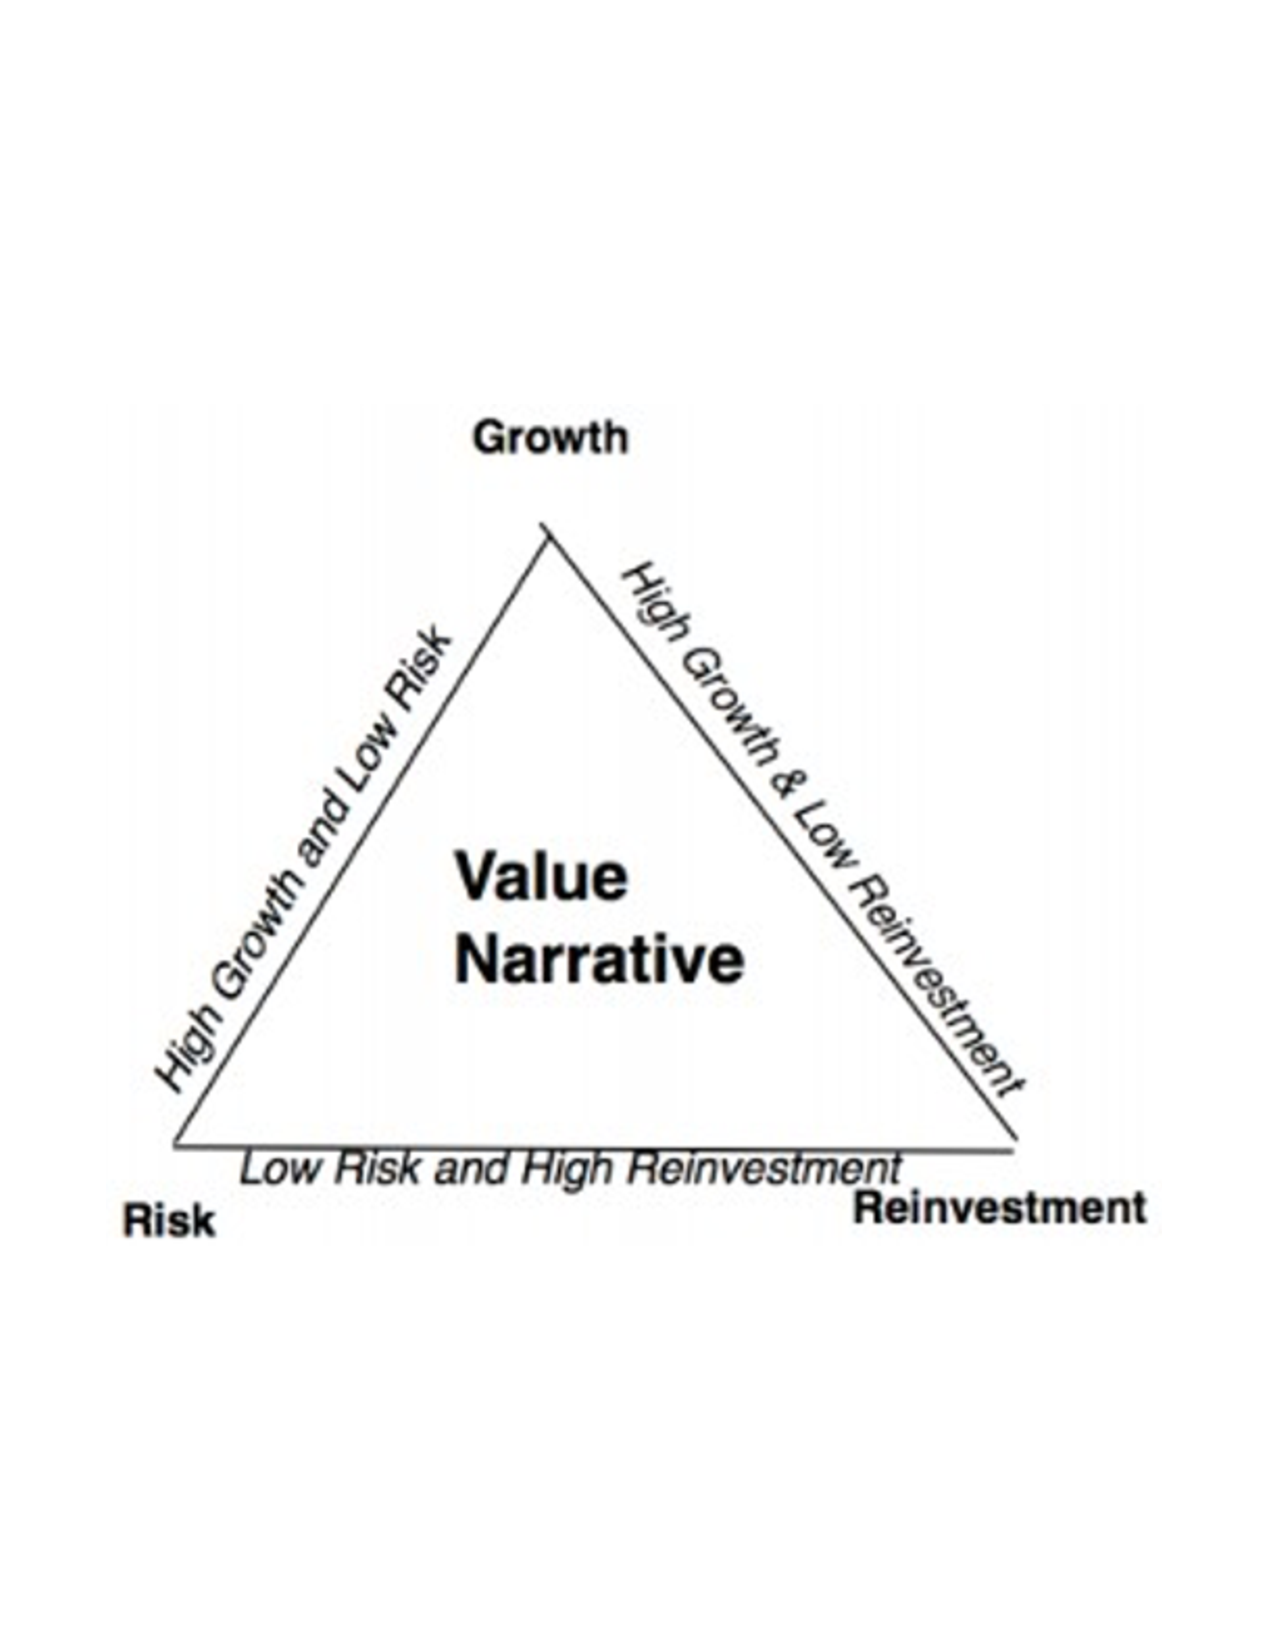
\includegraphics[height=5.5cm]{\rutaImagenes/narrativa_valuatoria}\\
\footnotesize{Fuente:Damodaran, A. ``Session 14. Narrative to numbers''. NYU/STERN.}

\end{minipage}

\end{figure}

\begin{enumerate}[i)]
\item \textcolor{secundario}{\gls{wacc} (costo promedio ponderado de capital).} El costo de capital es la compensaci\'on que los inversionistas exigen de parte de las firmas que utilizan sus fondos (costo de oportunidad).
\item \textcolor{secundario}{\gls{wara} (rendimiento del promedio ponderado de los activos).}Representa el promedio ponderado de las tasas de retorno de los Activos contributivos involucrados en la estimaci\'on del  valor razonable de un activo intangible.
\end{enumerate}

\begin{figure}[H]
\centering
\caption{Tasa de descuento WACC \& WARA.\label{fig:wacc_wara}}
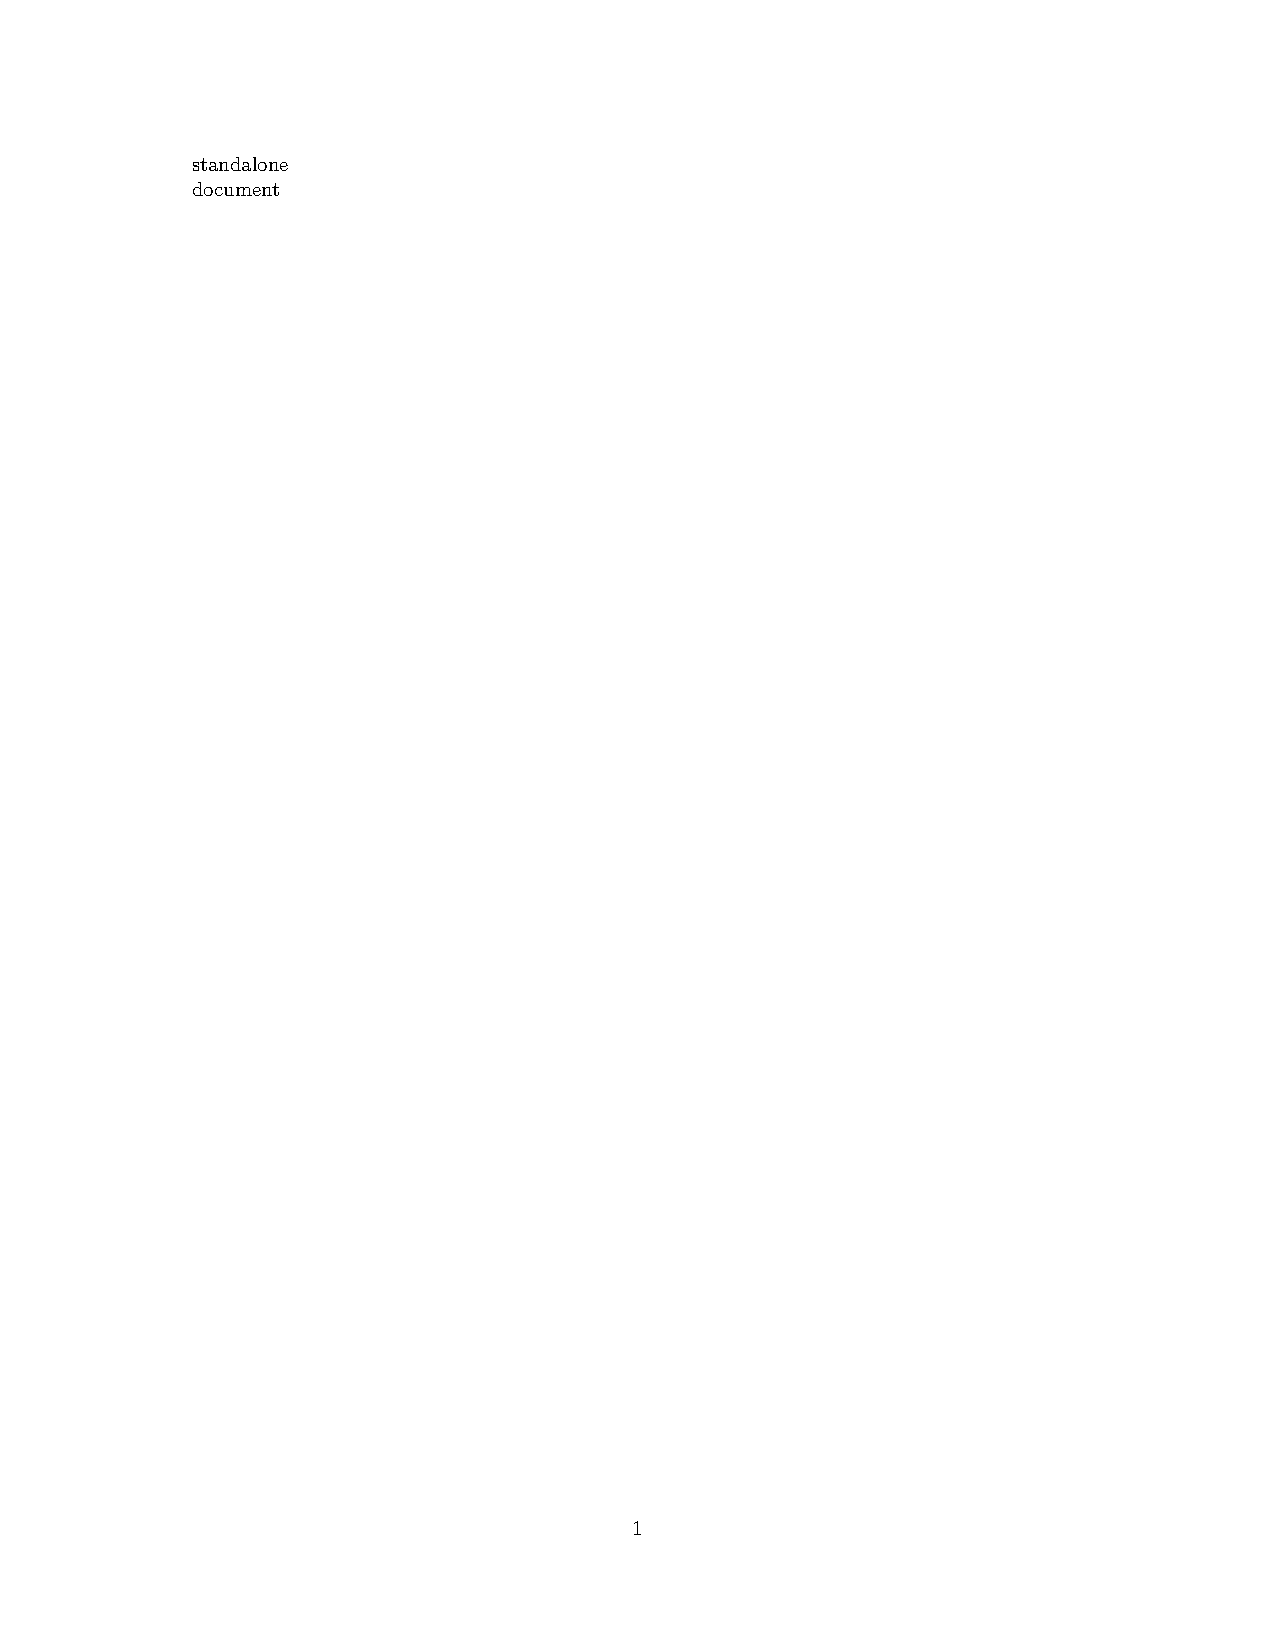
\includegraphics[width=12cm]{\rutaImagenes/wacc_wara}
\end{figure}
\textcolor{secundario}{CAPITAL ASSET PRICING MODEL (CAPM).} The underlying principle of the \gls{capm}  dictates that shareholders should earn at least a risk-free rate on their investment, plus a premium that compensates for the systematic risk of that investment.\\[10pt]

The formulation of the model is detailed below:\vspace{10pt}

\begin{center}
\begin{minipage}{8cm}
\begin{itemize}
\small
				\item The cost of equity capital is estimated using thel \textit{Capital Asset Pricing Model} (\gls{capm}):
				$$Rk=Rf+\beta\times(ERP)+SP+RP$$
				 \item Where:
				 \item $Rf$= Risk-free rate
				 \item $ERP$= Enterprise Risk premium
				 \item $\beta$=\gls{beta}
				 \item $SP$= Size Prime
				 \item $RP$ = Country Risk Prime
			\end{itemize}
	\footnotesize{Source: Valuaci\'on de Activos Intangibles. DEAL ADVISORY MEXICO. KPMG C\'ARDENAS DOSAL, S.C. KPMG ``D.R.''\copyright 2016.}
		\end{minipage}
\end{center}


\textcolor{secundario}{\textbf{Valuaci\'on Relativa (\textit{Relative Valuation}).}}\\[5pt]

El perito valuador aplic\'o la metodolog\'ia conocida como Valuaci\'on Relativa (Relative Valuation), mediante el modelo conocido como \gls{peers}, conforme al enfoque de mercado.\\




%\begin{figure}
%\caption{Modelo de Valuaci\'on Relativa.\label{fig:peers1}}
%
\includegraphics[width=8cm]{\rutaImagenes/peers_1}
%\end{figure}
%
%\begin{figure}
%\caption{PEERS m\'as Utilizados.\label{fig:peers2}}
%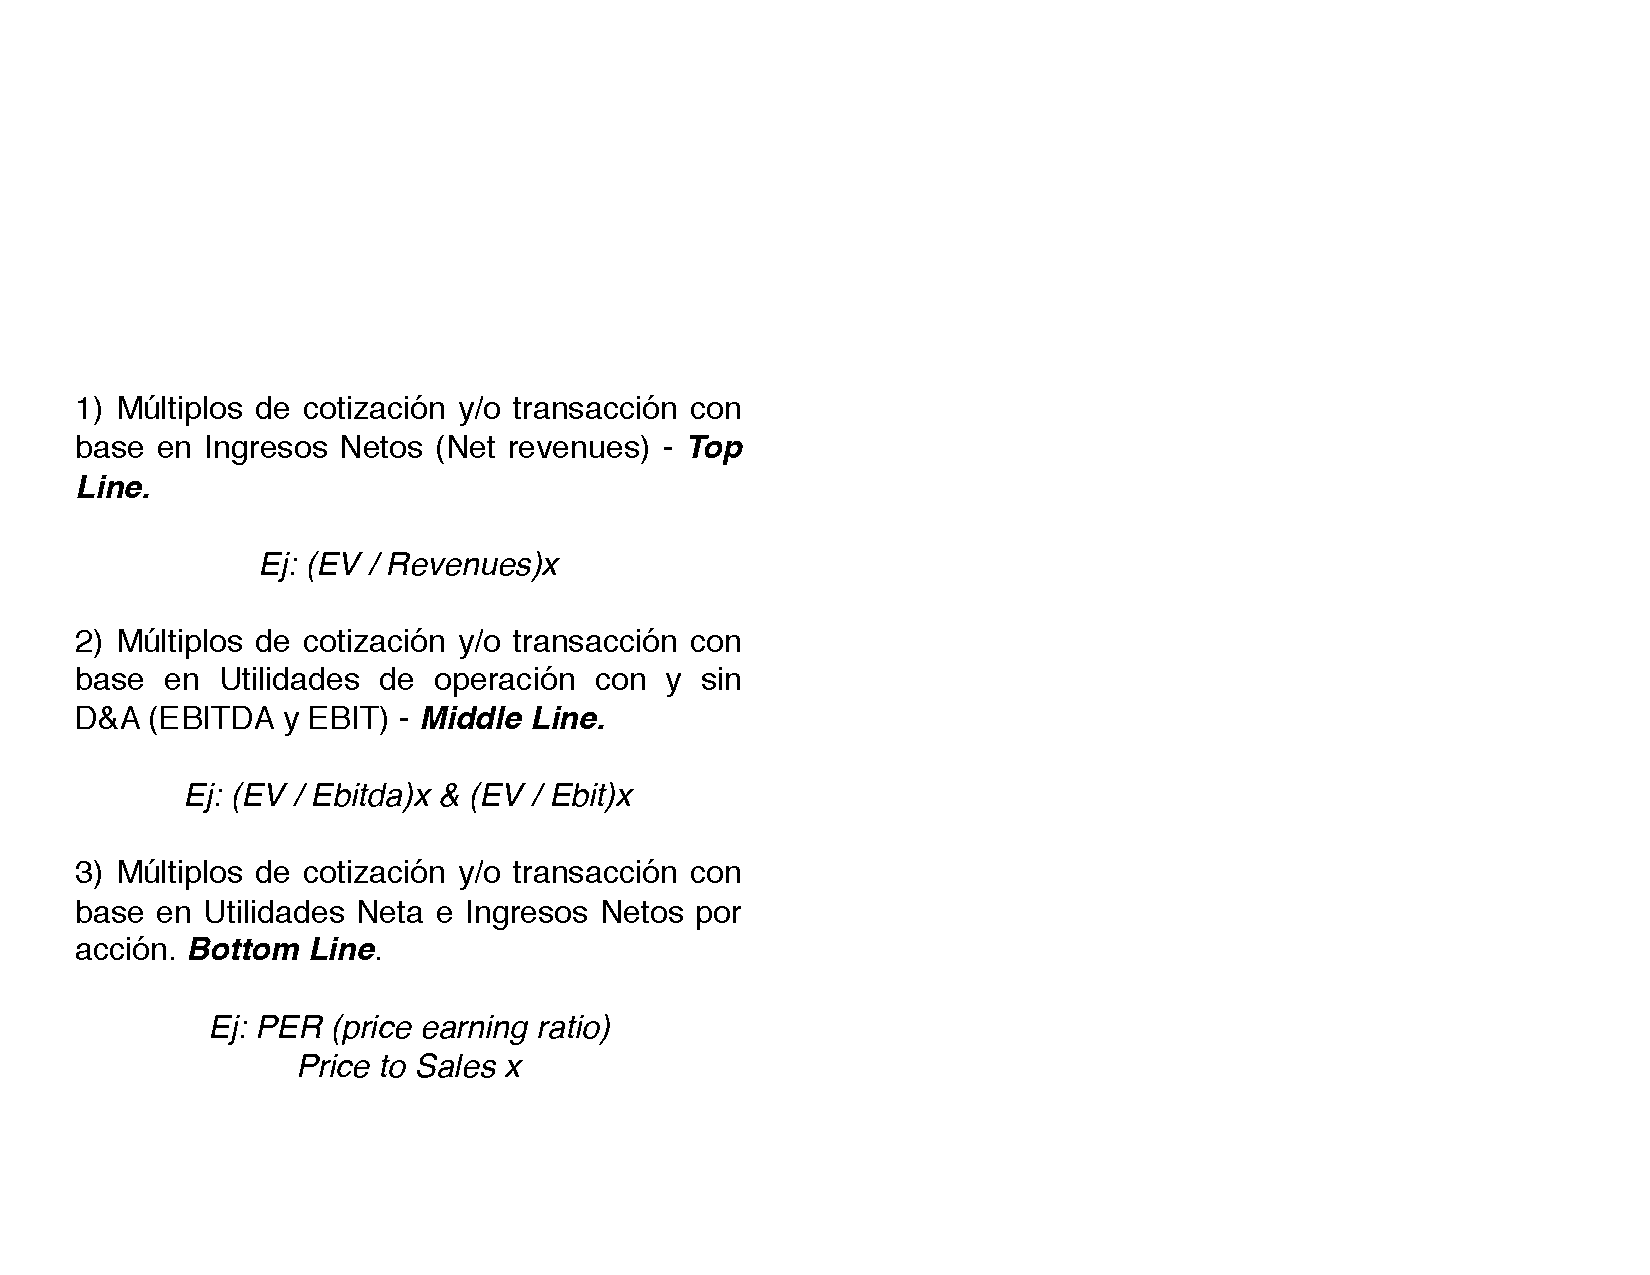
\includegraphics[width=8cm]{\rutaImagenes/peers_2}
%
%\end{figure}
\begin{figure}[H]
\caption{Modelo de Valuaci\'on Relativa. PEERS m\'as utilizados\label{fig:peers1}}
 \raisebox{-0.5\height}{
\includegraphics[width=6cm]{\rutaImagenes/peers_1}}
       \hfill
       \raisebox{-0.5\height}{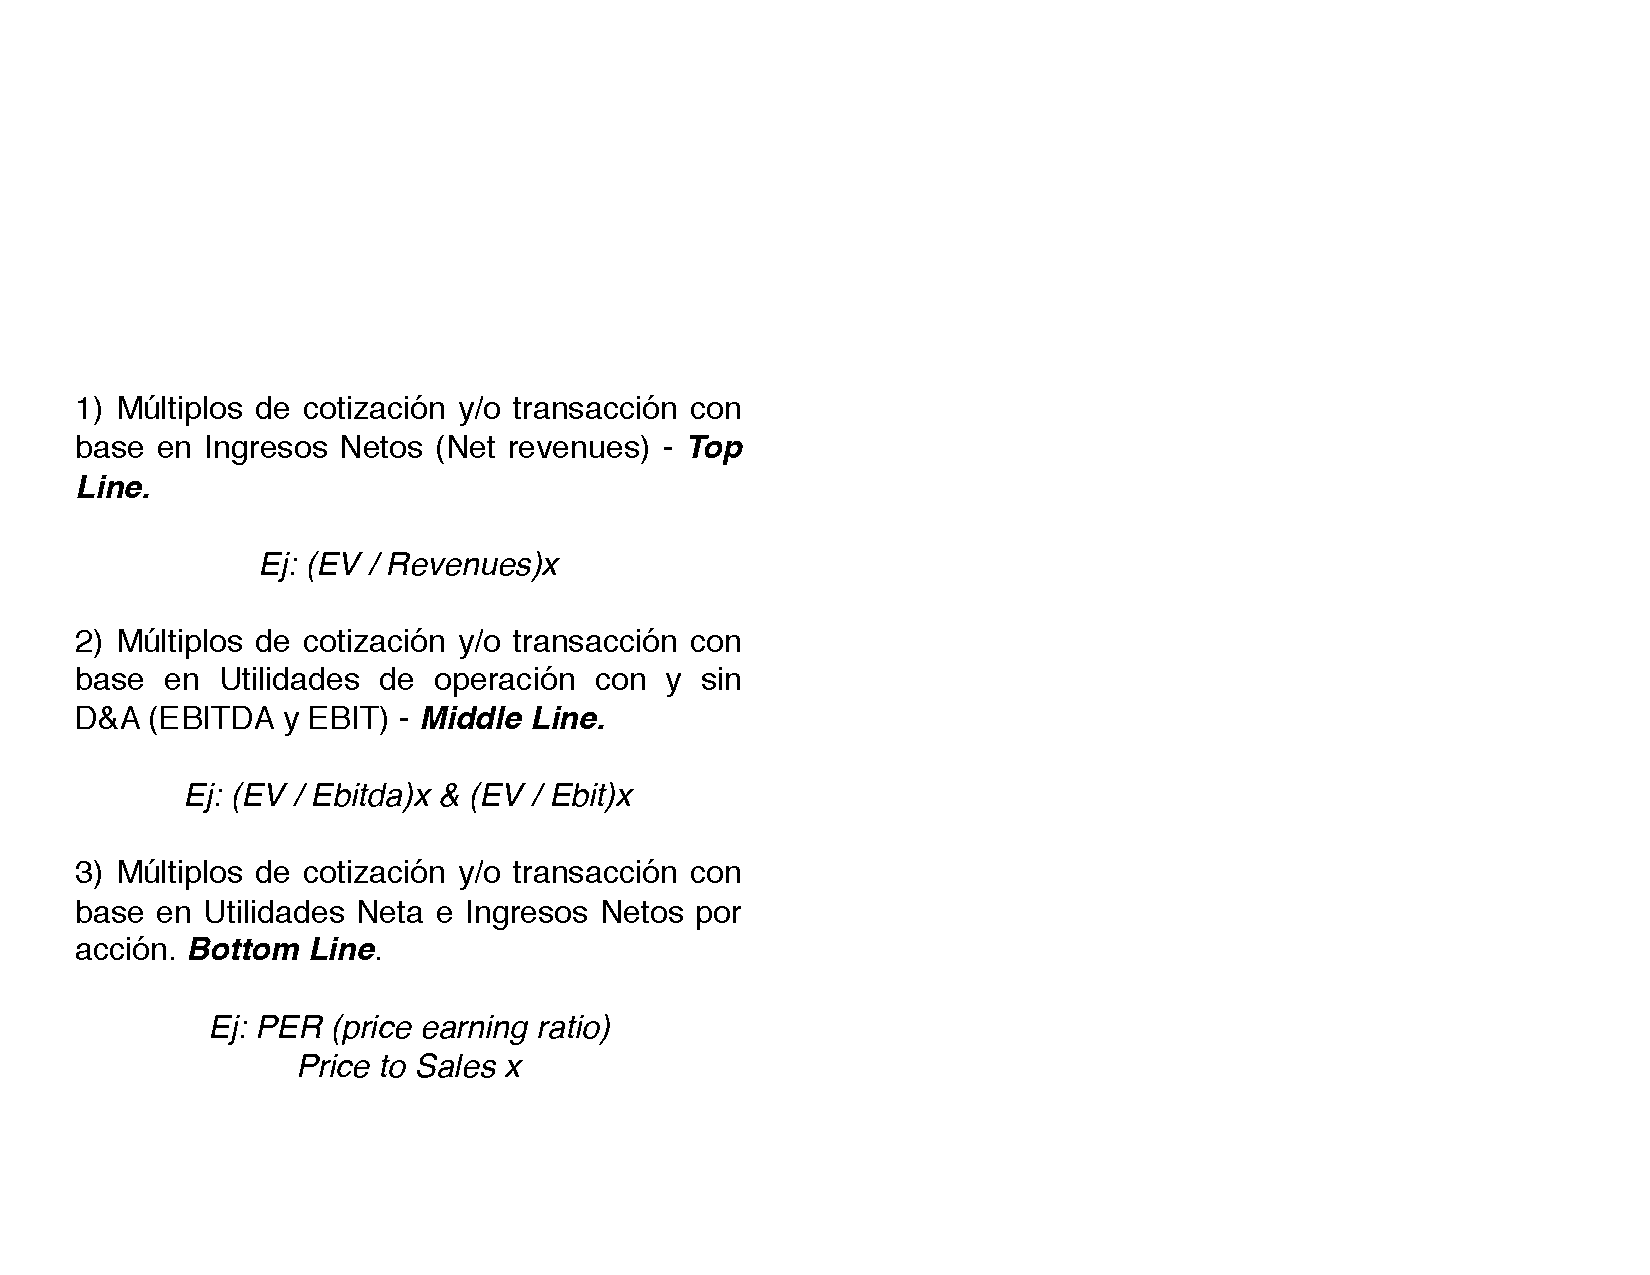
\includegraphics[width=8cm]{\rutaImagenes/peers_2}}
\end{figure}

 Esta metodolog\'ia permite determinar el valor de empresas no cotizadas en bolsa y en el caso de que la empresa objeto de valoraci\'on sea cotizada, el m\'etodo puede ayudarnos a detectar si el mercado  est\'a sobre o infravalorando el valor en cuesti\'on.  A su vez, permite determinar en una valuaci\'on financiera el componente de valor por enfoque de mercado (\textit{\gls{marketaproach}}), utilizando una muestra representativa sobre el m\'ultiplo  id\'oneo para el sujeto de valuaci\'on. \\
 
\textcolor{secundario}{INCOME APPROACH. Direct Capitalization Valuation Method. }\\


A \textcolor{principal}{perpetuity} is an infinite series of cash flows over time.\\

\textcolor{principal}{Perpetuities} are similar to annuities, in that they are payments of equal amounts made at equal time intervals, the difference being that the payments or installments of perpetuities are forever, as their name suggests.\\

This tool is especially useful for valuing companies and, therefore, their shares, given their nature of having ``perpetual life''. Some investments, like preferred stocks and bonds, are essentially perpetuities, and to transfer these assets from investors to other investors, they need to have a present value.
A perpetuity can be simple, if the cash flows are constant over time, or growing, if they increase over time:\\


\begin{center}
\begin{figure}[H]
\centering
	\caption{Direct Capitalization using Growing Perpetuity \label{fig:cap_dir}}\vspace{10pt}
	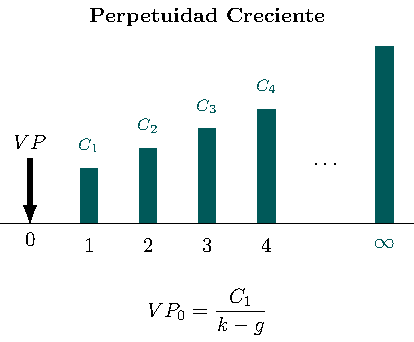
\includegraphics[width=5cm]{\rutaImagenes/capitalizacion_directa}\\
	
	\begin{minipage}{5cm}
	Where
	\begin{itemize}
	

	
		\item $C_1$: Cash Flow
		\item $k$: Capitalization rate
		\item $g$: Growth rate
	\end{itemize}
	\end{minipage}
\end{figure}
\end{center}



\textcolor{principal}{Capitalization using a growing perpetuity} refers to the case where the value of an income stream shows a noticeable and consistent upward trend over successive annual periods. In terms of investments, this often translates into a situation where the anticipated annual return from the investment is consistently met or even exceeded from one year to the next. The concept also implies that this cash flow will continue into the foreseeable future if the investor chooses to retain the asset over many years.\\

Evaluating the potential for a growing perpetuity is often very important for investors who wish to acquire a given investment with the aim of holding that investment over several years. Part of the process of accurately assessing the presence of a growing perpetuity year over year involves considering changes in the overall state of the economy. This means that it may be necessary to adjust figures for a given year to offset the effect of inflation.\\[10pt]


\espacio{4cm}
%=================Semblanza======================
\addcontentsline{toc}{section}{Semblanza y Análisis de Industria.}
\includepdf[pages=-,pagecommand={\thispagestyle{fancy}},height=\textheight]{../0.semblanza_eng/semblanza}


\chapter{DEVELOPMENT OF THE APPRAISAL.}\label{cap:5}
\thispagestyle{fancy}

%-----------------------Desarrollo del avalúo en la especie------------------------------------
\setcounter{section}{11}

\subsection{DEVELOPMENT OF THE VALUATION.}\label{sec:k2}

%\subsubsection{An\'alisis Financiero}


Se recibieron los Estados financieros hist\'oricos de \EFde{} y a \EFhasta, por parte del  solicitante, seg\'un se muestran a continuaci\'on:

\begin{figure}[H]
\centering
\caption{Estados de Situaci\'on Financiera Hist\'oricos \EFdeHasta \label{fig:ESF}}
\includegraphics[width=12cm]{../0.imagenes/EF_activo}\\[5pt]

\end{figure}
\begin{figure}[H]
\centering
\includegraphics[width=12cm]{../0.imagenes/EFpasivo_capital}\\

\end{figure}

\begin{figure}[H]
\centering
\caption{Estados de Resultados Hist\'oricos \EFdeHasta \label{fig:ESF}}
\includegraphics[width=12cm]{../0.imagenes/ER}\\
\end{figure}


Para el an\'alisis financiero de dicha empresa, se llevaron a cabo los siguientes m\'etodos:
\begin{enumerate}
\item An\'alisis del Capital Invertido (IC\footnote{Investment Capital}).
\item Razones financieras de liquidez y solvencia (Ratios bancarios).
\item An\'alisis Dupont de 3 elementos.
\item An\'alisis de la Rentabilidad del Capital (ROC\footnote{Return on Capital}).
\item An\'alisis de la Rentabilidad del Capital Operativo Neto (ROIC\footnote{Return on Investment Capital}).
\end{enumerate}

\begin{center}
\underline{An\'alisis del Capital Invertido (IC)}\\[10pt]
\includegraphics[width=12cm]{../0.imagenes/IC}\\[10pt]

\underline{Razones financieras de liquidez y solvencia}\\[10pt]
\includegraphics[width=12cm]{../0.imagenes/ratios}\\[10pt]

\underline{An\'alisis Dupont}\\[10pt]
\includegraphics[width=12cm]{../0.imagenes/dupont}\\[10pt]
\newpage
\underline{An\'alisis ROC}\\[10pt]
\includegraphics[width=12cm]{../0.imagenes/roc}\\[10pt]



\underline{An\'alisis ROIC}\\[10pt]
\includegraphics[width=12cm]{../0.imagenes/roic}\\[10pt]
\end{center}
 \subsubsection{Estimaci\'on de la Tasa de Descuento Ke.}

Cuanto mayor sea el riesgo sistem\'atico de una acci\'on, m\'as elevado ser\'a el rendimiento que los inversionistas esperar\'an de los t\'itulos accionarios. Con la finalidad de estimar una tasa de descuento apropiada en pesos, en t\'erminos nominales y despu\'es de impuestos, se utilizaron los siguientes insumos para determinar el valor de la \gls{wacc}:\\


\textcolor{principal}{Tasa libre de riesgo (Rf).} Se basa en el rendimiento de los bonos gubernamentales, en este caso, se tom\'o en cuenta el pronóstico del rendimiento del \textcolor{principal}{\rfBase}, con el siguiente resultado:

\begin{figure}[H]
\centering
La tasa libre de riesgo obtenida es de \textbf{\rfValor\%}\\[10pt]
 \includegraphics[width=9cm]{\rutaImagenes/banxico/cuadro_1_jul-ago_2023}
\end{figure}

\gls{beta}. Con la finalidad de determinar el factor \gls{beta} apropiado para el negocio, se consider\'o una muestra de mercado de \glspl{leveredbeta} de empresas comparables al negocio valuado:

\textcolor{principal}{Muestra de mercado de la beta del sector,  estructura de Deuda/Capital del sector (D/E), tasa efectiva de impuestos a la utilidad (ETR\%) :}

\espacio{4cm}
\begin{figure}[H]
\centering
\includegraphics[width=6cm]{../0.imagenes/beta_1}\\
\end{figure}

La beta apalancada de sector que corresponde a la empresa es de \textcolor{principal}{\textbf{\valorBeta x }(mediana)}\\

F\'ormula de BETA Despalancada:
\begin{figure}[H]
\centering
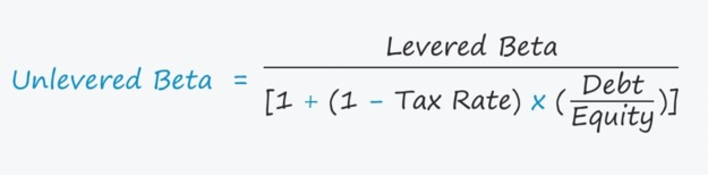
\includegraphics[width=8cm]{\rutaImagenes/beta_apalancada}
\end{figure}

El valuador llev\'o a cabo la estimaci\'on del pron\'ostico de BETA desapalancada al negocio, habiendo aplicado a la proporci\'on de deuda/capital del sujeto, el promedio de la muestra y la tasa fiscal efectiva del sector (ETR\footnote{Efective Tax Rate}); con un resultado de \textcolor{principal}{\betaDesapalancada x}.\\

F\'ormula de BETA Reapalancada:\\

\begin{figure}[H]
\centering

\includegraphics[width=8cm]{\rutaImagenes/beta_reapalancada}
\end{figure}

Una vez obtenido el indicador de BETA desapalancada del sector, el valuador llev\'o a cabo la estimaci\'on del pron\'ostico de BETA reapalancada al negocio sujeto de valuaci\'on, habiendo aplicado a la proporci\'on de deuda/capital del sujeto, la mediana\footnote{Conforme a la aplicaci\'on del rango intercuartil como medida de estandarizaci\'on}  de la muestra del sector y la tasa fiscal de M\'exico (MTR\footnote{Marginal Tax Rate}), con un resultado de \textcolor{principal}{\betaReapalancada x}\\



\textcolor{principal}{Prima de riesgo del mercado de capitales}. Se obtuvo del promedio hist\'orico de la diferencia de rendimientos o ``\textit{spread}'' entre el mercado accionario \mercadoAccionario{} mediante el indicador conocido como el \gls{erp} (\textit{enterprise risk premium}).\\

\begin{figure}[H]
\centering
La prima de riesgo de mercado (\gls{erp}) es de \textbf{\textcolor{principal}{\erpValor\%}} \\[10pt]

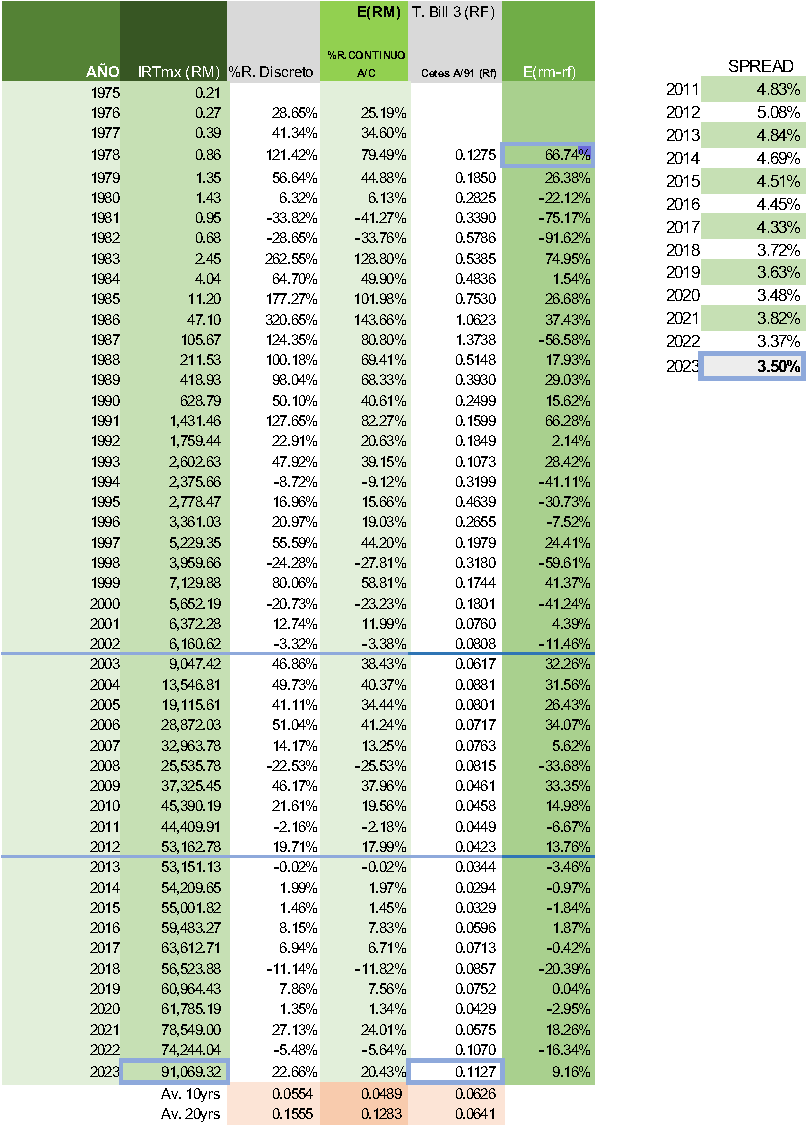
\includegraphics[width=5cm]{../0.imagenes/erp}
\end{figure}

%\textcolor{principal}{Riesgo Pa\'is (\gls{crp}).} Corresponde al riesgo pa\'is de M\'exico, seg\'un indicador de JP Morgan. Se considera un pron\'ostico para la prima de riesgo adicional de \crpValor{} puntos base.
%
%\begin{figure}[H]
%\centering
%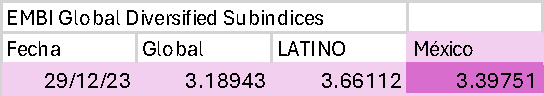
\includegraphics[width=8cm]{../0.imagenes/crp}
%\end{figure}

\textcolor{principal}{Prima por tamaño (\textit{Size Prime}).} \\[5pt]

Se tomo una prima por tamaño para la firma, a partir del valor en libros del capital contable de acuerdo a la siguiente tabla.\\

\textit{Nota. La tabla muestra la prima por tamaño a partir del valor en libros del capital contable en Millones de Euros.% Considerando el tipo de cambio  MEX/EUR a la fecha de valores de 20.8560 se obtiene un capital en euros por EUR 24,451,811.08.}
}

\begin{figure}[H]
\centering
La prima de tamaño es de \textbf{\textcolor{principal}{\sizePrime\%}} \\
\includegraphics[width=.8\textwidth]{../0.imagenes/size_prime_2}
\end{figure}


Estimaci\'on del costo de capital (\gls{ke}), con un resultado de \textcolor{principal}{\keValor\%.}

\begin{figure}[H]
\centering
\includegraphics[width=10cm]{../0.imagenes/ke}
\end{figure}


\textcolor{principal}{Costo de la deuda (\gls{kd}).} Para determinar la tasa \gls{wacc}, se consider\'o el costo impl\'icito de la deuda de la organizaci\'on, de acuerdo a par\'ametros de mercado de empresas similares:

\begin{figure}[H]
\centering
\includegraphics[width=10cm]{../0.imagenes/kd}
\end{figure}

\textcolor{principal}{C\'alculo del \gls{wacc}.} Como resultado de las consideraciones anteriores, se estima una \gls{wacc} en t\'erminos nominales y despu\'es de impuestos de \textcolor{principal}{\waccValor\%}.\\

\begin{figure}[H]
\centering
\includegraphics[width=12cm]{../0.imagenes/wacc}
\end{figure}


\subsubsection{RELATIVE VALUATION METHOD.}

\textcolor{principal}{Market Sample of Trading Multiples  (PEERS))}. The market approach was applied based on an indicator known as ``\textcolor{principal}{\peersa} x''; with an estimate of \textcolor{principal}{\peersaMult x} \footnote{\peersaEst{} of the sample} times \peersaTo:\\


%\begin{figure}[H]
%\centering
%
\includegraphics[width=11cm]{../0.imagenes/peers_1}
%\end{figure}

The market approach was also applied based on an indicator known as ``\textcolor{principal}{\peersb} x''; with an estimate of  \textcolor{principal}{\peersbMult x} \footnote{\peersbEst{} of the sample} times \peersbTo:\\

\begin{figure}[H]
\centering

\includegraphics[width=14cm]{../0.imagenes/peers_1}
\end{figure}

%\newpage
%
%Se aplic\'o el enfoque de mercado con base en un indicador conocido como ``\textcolor{principal}{\peersc} x''; con una estimaci\'on de \textcolor{principal}{\peerscMult x} \footnote{\peerscEst{} de la muestra} veces \peerscTo:\\
%
%\begin{figure}[H]
%\centering
%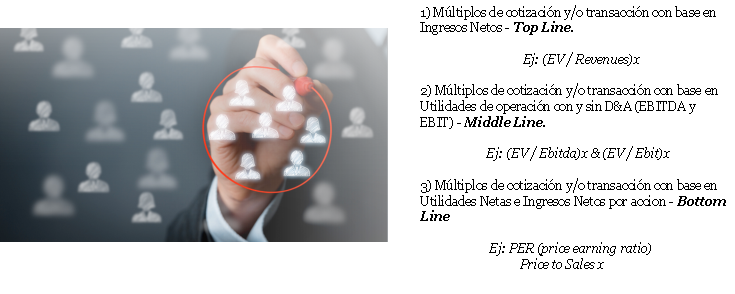
\includegraphics[width=11cm]{../0.imagenes/peers_3}
%\end{figure}
%
%\newpage
%
%Se aplic\'o el enfoque de mercado con base en un indicador conocido como ``\textcolor{principal}{\peersd} x''; con una estimaci\'on de \textcolor{principal}{\peersdMult x} \footnote{\peersdEst{} de la muestra} veces \peersdTo:\\
%
%\begin{figure}[H]
%\centering
%\includegraphics[width=11cm]{../0.imagenes/peers_4}
%\end{figure}
%
%\newpage
%
%Se aplic\'o el enfoque de mercado con base en un indicador conocido como ``\textcolor{principal}{\peerse} x''; con una estimaci\'on de \textcolor{principal}{\peerseMult x} \footnote{\peerseEst{} de la muestra} veces \peerseTo:\\
%
%\begin{figure}[H]
%\centering
%\includegraphics[width=11cm]{../0.imagenes/peers_5}
%\end{figure}



\subsection{Value of the Business by PEERS.} The appraiser conducted a capitalization by multiples for the estimation of the fair value of the company, according to the market approach; as can be seen:

\begin{figure}[H]
\centering
\includegraphics[width=.7\textwidth]{../0.imagenes_eng/valor_peers}\\

%Valor razonable por PEERS: \textcolor{principal}{\$\valorPeers MXN}
\end{figure}
\subsection{APPLICATION OF THE DIRECT CAPITALIZATION METHOD. Through the income approach.} 


After conducting a detailed financial analysis of the business and given the difficulty in accurately projecting the revenues and cash flows of the entity due to its current negative equity and the variability of its historical figures, the appraiser decided to capitalize the NOPAT of the business with figures as of 2023, using a nominal capitalization rate that represents the opportunity cost of the business, along with the minimum expected appreciation of the Mexican economy, also taking into account the growth of such cash flows at a long-term inflation rate; having used the model of Geometrically Growing Annuity in accordance with the theoretical framework of corporate finance:\\


\begin{figure}[H]
\centering
\includegraphics[width=9cm]{../0.imagenes_eng/cap_dir}
\end{figure}



\newcommand{\ponda}{Direct Capitalization)}
\newcommand{\pondaPorcentage}{33}
\newcommand{\pondb}{\peersa}
\newcommand{\pondbPorcentage}{33}
\newcommand{\pondc}{\peersb}
\newcommand{\pondcPorcentage}{33}
\newcommand{\pondd}{\peersd}
\newcommand{\ponddPorcentage}{30}
\newcommand{\ponde}{\peersd}
\newcommand{\pondePorcentage}{30}

\subsection{WEIGHTED FAIR VALUE OF THE ONGOING BUSINESS, WITH FIGURES AS OF \fechaValoresCorto.}


The fair value of the firm (Firm Value), as of the valuation date, is concluded next, having given the following importance to the models in the weighting: i) A weight of \pondaPorcentage\% to the valuation model known as \ponda{}, ii) A weight of \pondbPorcentage\%  to the relative valuation model (PEERS) known as \pondb{} x; iii) A weight of \pondcPorcentage\%  to the relative valuation model (PEERS) known as \pondc{} x; as shown below:

\begin{figure}[H]
\centering
\includegraphics[width=12cm]{../0.imagenes_eng/valor_ponderado_firma}\\

\textbf{\textcolor{principal}{Firm Value as of  \fechaValoresCorto:} \$\valorFirma{} MXN}\\[5pt]
(\textcolor{principal}{\valorFirmaLetra{} pesos 00/100 M.N.})
\end{figure}

%\newcommand{\valorCapitalM}{906}
%\newcommand{\valorCapitalm}{356}
%\newcommand{\valorCapitalc}{853}
%\newcommand{\valorCapital}{\valorCapitalM,\valorCapitalm,\valorCapitalc}
%\newcommand{\valorCapitalLetra}{\Numberstringnum{\valorCapitalM}{} millones, \numberstringnum{\valorCapitalm}{} mil, \numberstringnum{\valorCapitalc}}

\subsection{FAIR VALUE OF EQUITY CAPITAL, WITH FIGURES AS OF \fechaValoresCorto}

Once the value of the business firm was estimated, the appraiser proceeded to subtract the Net Debt of the business, thus obtaining the fair value of the equity capital.\\

Next, the fair value of the equity capital (\textit{\gls{equityvalue}}) as of the valuation date is concluded:\\


\begin{figure}[H]
\centering
\textbf{\textcolor{principal}{Equity Capital Value as of \fechaValoresCorto:} \$\valorCapital{} MXN}\\
\includegraphics[width=8cm]{../0.imagenes_eng/valor_cap_acc}\\
(\textcolor{principal}{\valorCapitalLetra{} pesos 00/100 M.N.})


\end{figure}

\subsection{Fair Value per Share.}

At the express request of the applicant, the appraiser proceeded to calculate the fair value corresponding to each share. Therefore, the number of shares available was first accounted for (according to the information provided by the applicant), and then the total fair value of the Equity was divided by the number of shares; thus obtaining a  \textcolor{principal}{unit value per share of \$328.19 pesos per share}, as can be seen:

\begin{figure}[H]
\centering
\includegraphics[width=12cm]{../0.imagenes_eng/valor_por_accion}\\

\textbf{\textcolor{principal}{Conclusion:}}\\

\textbf{\$328.19 MXN}\\
(\textcolor{principal}{Three hundred twenty-eight pesos 19/100 M.N.})
\end{figure}

%-----------------------FECHA DE INSPECCIÓN---------------------
\section{INSPECTION DATE}\label{sec:l}
Not applicable.

%------------------------FECHA DE VALORES------------------------
\section{REFERENCE DATE FOR VALUE}\label{sec:m}
\fechaValores.

%-----------------------FECHA DEL INFORME-----------------------
\section{VALUATION REPORT DATE}\label{sec:n}
\fechaInforme.

%----------------------FUENTES DE INFORMACIÓN--------------
\section{SOURCES OF INFORMATION}\label{sec:nn}
\begin{itemize}

\item To obtain economic data for Mexico such as inflation, please consult the website of the National Institute of Statistics and Geography (INEGI): \url{http://www.inegi.org.mx/sistemas/IndicePrecios/}

\item For financial information related to industry, sector, discount rates, and peers, you can visit: \url{https://www.refinitiv.com/en}

\item To access reference data on risk-free rates for Mexico, please refer to the website of the Bank of Mexico: \url{www.banxico.org.mx}

\item For obtaining macroeconomic indicators, you can find information from ``Economía en breve'' by Mtro. Mario Correa at: \url{https://www.youtube.com/channel/UCtt93euOsTuq_gjUiZV-MSA}

\item For other financial data, you can visit the following websites:
\begin{itemize}
\item\url{www.damodaran.com}
\item \url{www.reuters.com}
\item \url{www.bmv.com.mx}
\item \url{www.sat.gob.mx}
\end{itemize}

\item For sector analysis, brand profiles, and the macro environment, you can access Passport Euromonitor at: \url{https://www.portal.euromonitor.com/}
\begin{itemize}
\item \url{https://www.vivo.com/en}
\item \url{https://www.vivo.com/mx}
\item \url{https://www.statista.com/statistics/541618/vivo-smartphone-shipments-worldwide/}
\item Vivo share of global smartphone shipments 2019-2023. Statista
\item Vivo Communication Technology. Crunchbase Company Profile \& Funding
\item La venta de ``smartphones'' mueve 93.000 millones hasta marzo: qué marcas suben y cuál se desploma? \url{elpais.com}
\end{itemize}
	 
\end{itemize}
%-----------------------CONSIDERACIONES PREVIAS A LA CONCLUSI\'ON------------------
\section{PRELIMINARY CONSIDERATIONS BEFORE CONCLUSION}\label{sec:o}
\begin{enumerate}
	\item El presente estudio s\'olo es v\'alido para el prop\'osito y uso que se indica en los incisos \ref{proposito} e \ref{uso} de este dictamen y cuando cuente con la firma \ifthenelse{\equal{\peritoAuxiliar}{n/a}}{del perito valuador}{de los peritos valuadores}.
	\item Las declaraciones de hechos, datos y documentos proporcionados por el solicitante para la realizaci\'on de este informe, se asumen como verdaderas y correctas.
	\item El an\'alisis y opiniones reportados en el presente dictamen est\'an limitados s\'olo por las suposiciones y condiciones limitantes reportadas y son el resultado de las conclusiones profesionales e imparciales  \ifthenelse{\equal{\peritoAuxiliar}{n/a}}{del valuador que firma}{de los valuadores que firman}.
	\item  \ifthenelse{\equal{\peritoAuxiliar}{n/a}}{El perito valuador que firma no tiene}{Los peritos valuadores que firman no tienen}{} inter\'es presente o futuro en las cifras conclusivas de las que es objeto de este informe, ni tampoco  \ifthenelse{\equal{\peritoAuxiliar}{n/a}}{tiene}{tienen}{} intereses personales o parcialidad con respecto a las partes involucradas.
	\item La compensaci\'on econ\'omica  \ifthenelse{\equal{\peritoAuxiliar}{n/a}}{del perito valuador}{de los peritos valuadores}{} no est\'a condicionada al informe de un valor predeterminado o dirigido a un valor que favorezca la causa del solicitante.
	\item Este dictamen valuatorio s\'olo podr\'a ser usado \'integro y no en partes. Ninguna parte del reporte podr\'a ser utilizada en conjunto a alg\'un estudio ajeno al mismo. La publicaci\'on del mismo o cualquiera de sus partes, sin la autorizaci\'on escrita del suscrito Corredor P\'ublico est\'a prohibida. Este aval\'uo no podr\'a ser usado por ninguna persona o entidad distinta a la que est\'e dirigida o para un prop\'osito o fin distinto al estipulado.
	\item El presente estudio no valida o se\~nala el tratamiento jur\'idico, contable y/o fiscal de las cifras conclusivas del informe; conforme a las normas de informaci\'on financiera (NIF), la ley del ISR, la Ley del IVA y dem\'as normatividad aplicable.

\end{enumerate}

\chapter{CONCLUSIONS.}\label{cap:6}
\thispagestyle{fancy}
%-----------------------CONCLUSIÓN DE LA VALUACIÓN-----------------------
\setcounter{section}{16}
\section{VALUATION CONCLUSION.}\label{sec:p}
\textcolor{principal}{\underline{UNICA.-}} El \textcolor{principal}{VALOR RAZONABLE} de la sociedad \textcolor{principal}{\empresaSolicitante} como negocio en marcha (\textit{\gls{firmvalue}}), as\'i como de su capital accionario (\gls{equityvalue}) conforme a la aplicaci\'on de los modelos de valuaci\'on descritos en los cap\'itulos \ref{cap:4} y \ref{cap:5}  de este dictamen, con fecha de valores al \fechaValores, seg\'un el prop\'osito y uso del aval\'uo, es por la siguiente cantidad:\\

\begin{figure}[H]
\centering
\textcolor{principal}{Valor de la Firma al \fechaValoresCorto:}\textbf{\$\valorFirma{} \monedaCode}\\

(\textcolor{secundario}{\valorFirmaLetra{} \moneda{} 00/100 M.N.})

\includegraphics[width=12cm]{../0.imagenes/valor_ponderado_firma}\

\textcolor{principal}{Valor del Capital Accionario al \fechaValoresCorto:} \textbf{\$\valorCapital{} \monedaCode}\\
(\textcolor{secundario}{\valorCapitalLetra{} \moneda{} 00/100 M.N.})\\
\end{figure}

\begin{figure}[H]
\centering
\includegraphics[width=7.5cm]{../0.imagenes/valor_cap_acc}

\end{figure}
\espacio{.5cm}

\vspace{2cm}

A mi mejor juicio y parecer, siendo los \textcolor{principal}{\diainforme{} d\'ias del mes de \monthname[\mesinforme]{} del a\~no \annoinforme (\numberstringnum{\annoinforme})} seg\'un el criterio valuatorio explicado en el desarrollo de este dictamen, expido el presente \textcolor{principal}{DICTAMEN VALUATORIO}, con \textcolor{principal}{\textbf{FECHA DE VALORES}} al d\'ia \textcolor{principal}{\textbf{\fechaValores}}; para todos los efectos a que haya lugar.\\

\begin{table}[H]
\centering
	\begin{tabular}{c}
	\begin{minipage}{7cm}
	\begin{center}
		``PERITO VALUADOR''\\[1cm]
		
		\rule{7cm}{.4pt}\\
		\nombrePerito\\
		\textcolor{principal}{\descripcionFirmaPerito}
		
	\end{center}
	\end{minipage}
	
	\end{tabular}
\end{table}
%----------------------REPORTE FOTOGRAFICO------------------------------
\section{PHOTOGRAPHIC REPORT}\label{sec:q}
Not applicable.
%---------------------ANEXOS-------------------------------------------------------- 
\section{APPENDIX}\label{sec:r}

Appendix 1.- Corporate Information. Appendix 2.- Financial Information.



\label{lastpage}
\end{document}
